% !TEX TS-program = pdflatex
% !TEX encoding = UTF-8 Unicode
% arara: pdflatex: { draft: true }
% arara: biber
% arara: pdflatex: { synctex: true }
% arara: pdflatex: { synctex: true }
\documentclass[11pt]{article}
\setcounter{secnumdepth}{5}

\usepackage{listings}
\lstset{% Add other global options here
  escapechar=\&% char to escape out of listings and back to LaTeX
} 
\usepackage{caption,subcaption}
\usepackage{float}
\restylefloat{table}
\usepackage[swedish]{babel} % Enables swedish typesetting, needs to be at top of document
\usepackage[T1]{fontenc}
\usepackage[utf8]{inputenc} % set input encoding (not needed with XeLaTeX
\usepackage{textcomp} % Suppress unicode char error
\usepackage{enumitem} % resume numbering in enumerations
\usepackage[bottom = 110pt]{geometry} % to change the page dimensions
%\geometry{a4paper} % paper format, could also be placed in documentclass options
\usepackage{graphicx} % support the \includegraphics command and options
\usepackage[parfill]{parskip} % Begin paragraphs with an empty line rather than an indent
\usepackage{verbatim} % adds environment for commenting out blocks of text & for better verbatim
%\usepackage{titling} % required for setlength droptitle (below)
%\setlength{\droptitle}{-70pt} % Adjust title height
\usepackage{fancyhdr} % This should be set AFTER setting up the page geometry
\pagestyle{fancy} % options: empty , plain , fancy
%\renewcommand{\headrulewidth}{0pt} % customise the layout...
%\lhead{}\chead{}\rhead{} % fancyhdr style reset for header
\usepackage{fancyvrb}
%\lfoot{}\cfoot{\thepage}\rfoot{} % fancyhdr style reset for footer
%\usepackage{sectsty} % Section title
\usepackage{hyperref} % href
\usepackage{caption}
\usepackage{subcaption}
\usepackage{nameref} % Enable referring to the actual name of the chapter
\usepackage[style=authoryear,backend=biber,maxcitenames=1]{biblatex}
\renewcommand*{\labelnamepunct}{\addcolon\space}
\bibliography{references.bib}
\usepackage{url}

\title{Mobile-first eller Desktop-first, en studie om utvecklingslösningar för responsive web design}
\author{Eduardo Castaneda}
%\date{} % Uncomment to hide date, or provide a date to display


\pagestyle{fancy}               % Fräcka sidhuvuden
\addtolength{\headwidth}{0cm}   % Sidhuvd bredare än texten.
\renewcommand{\headrulewidth}{0.4pt}
\renewcommand{\footrulewidth}{0.4pt}

\begin{document}

\maketitle
\thispagestyle{empty}


\newpage

\begin{abstract}

I examensarbetet analyseras mobile-first och desktop-first vilka är två olika tillvägagångssätt för responsiv web design. Responsiv web design är ett koncept för webbsidor vars design anpassas utifrån skärmstorlek. Analysen utförs genom att samla in synpunkter kring metoderna och analysera användnindsområdet för mobilt och desktop internet för att skapa en prototyp av en responsive webbplats där båda metoder utförs.

Den största skillnaden mellan metoderna är att grunden är avsedd för mobilen respektive skrivbordskärmen. Arbetet visar att mobile-first ger ett bättre resultat för mobilen, vilken tillskillnad från en dator har sämre prestanda, mindre skärm och sämre internetuppkoppling,
därav en fördel för den enhet som behöver fokus för att upprätthålla snabb respons. Desktop-first tar inte det i akt, utan fokus sker för datorn där prestandan är så pass hög att skillnaden för responsen är liten. Resultat visar även det naturliga arbetssättet mobile-first tillför då designen för mobilen utvecklas utifrån en perspektiv som är standard inom webbutveckling. Desktop-first har fördelen att vara ett snabbt tillvägagångsätt för att skapa responsivt utifrån en existerade webbsida, men kommer däremot att sakna den stabila grund mobile-first kan uppnå.

Implementationen av prototypen har inte kunnat styrka alla påståenden kring metoderna. Men ändå kunnat styrka tillräckligt många för att lyfta mobile-first som den metod som gynnar utvecklingen av responsiva sidor och den utveckling som sker inom internetanvändning. En utveckling där mobilt internet ökar markant och fler webbsidor ses utifrån mobilen. 



\end{abstract}
\thispagestyle{empty}

\newpage
\tableofcontents
\newpage


\section{Inledning}
Användningen av mobilt internet ökar för varje dag och nya webblösningar har krävts för att nå ut till mobilanvändarna. En av lösningarna har varit responsive web design. Responsive web design innebär att samma webbsida rendereras olika beroende på enheten webbsidan ses från och kan på så sätt anpassas utifrån skärmstorleken. Tekniken för att skapa responsiva webbsidor existerar, med hjälp av utvecklingen av tekniker och verktyg så som CSS, HTML finns i nuläget möjligheten att skapa webbsidor som beroende på skärmstorlek har olika designlayouts med en och samma kodgrund. Det finns även kunskap om tillvägagångsätt för skapandetav responsiva webbsidor, där utvecklare med formler och riktlinjer kan lära sig att använda grundprinciperna fluid grid, fluid images och media queries på bästa sätt. Däremot är vägen till att skapa en responsiv webbsida olika.  I bloggar och forum på webben diskuteras flitigt valet av utvecklingsmetod när det kommer till responsiva webbplatser och innan implementeringen av en webbsida är detta en fråga som med stor sannolikhet dyker upp hos webbutvecklare. Utvecklingsmetoderna som diskuteras är \textit{Mobile-first} och \textit{Desktop-first}. Mobile-first och Desktop-first är två olika metoder där det responsiva angreppssättet används. Båda strävar efter samma mål, men skiljer sig i implementeringen för responsive web design.

\subsection{Mobile-first eller Desktop-first}
Kännetecken för metoderna är  grunden på strukturen och designen,  där storleken på webbläsaren avgör på vilket sätt den  skall ändras för att anpassas för en annan enhet. Kunskapen om metoderna var för sig har med tiden blivit större i samband med utvecklingen av responsive web design. Däremot ställs webbutvecklare kring frågan om vilken metod som appliceras bäst till typen av webbsida som skall skapas. I dagsläget finns ingen kunskap om hur bra metoderna appliceras i jämförelse med varandra. Det finns tankar och spekulationer, därefter väljs metod utifrån dessa, komplikationer hanteras men dokumenteras inte vilket tillslut leder till en fungerande webbsida utan vetskapen ifall bästa lösning är applicerad. Eftersom webbsidan är färdig implementerad finns ingen anledning till att implementera om en fungerande lösning med en annan metod, därav finns ingen större kunskap om jämförelse av implementationen med respektive metod riktat mot ett och samma resultat.

Användning av mobilt internet ökar och användningen av internet via en dator kommer med stor sannolikhet bestå. Det gör att en grund för val av metod är högst passande, då det redan nu och i framtiden kommer att kräva mer kunskap än vad som idag kan erbjudas från bloggar. Båda metoder har sina fördelar samt nackdelar, vilket bör lyftas fram tydligare. Frågan som även bör ställas är när metoderna utnyttjas på bästa sätt och kan valet av metod leda till positiva faktorer vilka motsatta metod inte hade kunnat uppnå.

\begin{figure}[h]
\centerline{%
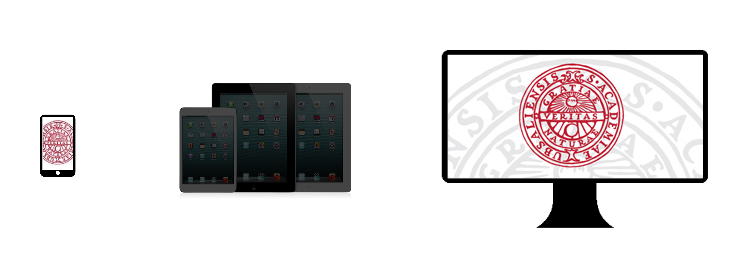
\includegraphics[scale=0.6]{pics/olikaenheter.png}
}
\end{figure}
\vspace{1.5cm}
Figur 1: En responsive webbsida kan även anpassas till enheter mellan desktop och mobil, t.ex  tablets och ipads.  I arbetet kommer fokus endast ske för mobil och desktop.


\subsection{Valtech AB}
Examensarbetet kommer att utföras på Valtech AB i Stockholm. Valtech Sverige fokuserar främst på utveckling av användaranpassade webbsidor, webbapplikationer och intranät. Hos Valtech finns erfarna gränssnittsutvecklare som har stött på problem under utvecklingsprocessen i form av ett beslutstagande av tillvägagångssätt för en responsiv webbsida. Det finns ett behov hos utvecklare på Valtech att ha en grund för vilka faktorer som är viktigast vid beslutstagande för metod och som ger den bästa lösning för en effektiv utveckling av en responsiv webbplats. Gränsnittssutvecklarna besitter på mycket erfarenhet och kunskap, vilket kan samlas och användas som vägledning för att finna problem som uppstår i verkliga situationer.

\subsection{Syfte}
Syftet med arbetet är att kunna hitta riktlinjer till när en specifik metod appliceras bäst. Det vill säga beroende på faktorer kring webbsidan hitta den metod som tillför det mest optimala lösningen för implementationen av en webbsida. Att hitta en metod som fungerar bäst i alla lägen är inte nödvändigtvis målet med arbetet då det existera många olika vinklar, vilka gör det svårt att hitta en specifik metod som ger det optimala resultatet oberoende på situation.

\vspace{0.5cm}
Frågeställningar som besvaras i rapporten är:
\begin{enumerate}
	\item I vilka lägen appliceras metoderna bäst?
	\item Vad är för- och nackdelarna med Mobile-first?
	\item Vad är för- och nackdelarna med Desktop-first?
\end{enumerate}
\vspace{0.5cm}
\textit{Frågeställning 1} baseras på miljö, målgrupp och kontext. Syftet med frågeställningen är att kunna utifrån analys hitta situationer där metoderna visar sig vara fördelaktiga under utvecklingsfasen, för att hitta faktorer hos metoden vilka motsatta metod inte har och därmed inte kan tillföra samma lyckade resultat. Syftet med \textit{Frågeställning 2 och 3} är att kunna lyfta fram de fördelar och nackdelar som finns vid implementation med de två metoderna. För att på så sätt hitta ramar för varje metod vilka en läsare kan relatera till med en egen situation och utifrån det använda det som grund vid val av metod. 

\subsection{Avgränsningar}

Arbetet kommer att enbart fokusera på mobile-first och desktop-first \textit{(se figur 1)}. Ett mellanläge som existerar för Ipads, tablets, osv. kommer inte att tas med i arbetet utan kommer att ses som desktopläge. I dagsläget finns även andra lösningar för mobilt webb t.ex \textit{Appar} och \textit{separata mobilsidor}, jämförelse mellan dessa och responsive web design kommer inte att göras, utan jämförelsen som görs är mellan mobilalösningar inom responsive web design.

Termen \textit{Mobile-first} kan tolkas på olika sätt. Det har förekommit tillfällen för webbutvecklare där mobile-first är prioriterad designmässigt men där implementeringen ändå har skett för desktop innan mobilen. Det är inte fallet i arbetet, utan mobile-first beskrivs som en tanke och en implementering avsedd för mobilen i första hand, och tvärtom för desktop-first.

\subsection{Disposition}

Kommande kapitler är indelade i \textit{Bakgrund}, \textit{Teori}, \textit{Metod}, \textit{Resultat} och \textit{Diskussion}. I \textit{bakgrund} beskrivs den ökning av användning som har skett för mobilt internet under de senaste åren och även användningen av desktop internet som har bestått. I bakgrund beskrivs även betydelsen dessa har för webbutvecklingen och varför responsive web design är en metod som kan gynna dem. I kapitlet \textit{teori} förklaras tekniken responsive web design samt de verktyg och metoder som samverkar för att få en fungerande responsiv webbplats, på så sätt tillföra en teknisk förståelse för hur webbutvecklingen av mobile-first och desktop-first går till. Metoderna för arbetet är en litteraturstudie samt en prototyp av en webbsida som både implementeras i mobile-first och desktop-first. I kapitlet \textit{metod} beskrivs valet av metoderna samt hur dessa samspelas för att få fram resultat som besvarar frågeställningarna för arbetet. I nästa kapitel, \textit{resultat}, samlas resultatet från tillvägagångsätten som beskrivs i metod, vilket senare diskuteras i kapitlet \textit{diskussion}, där även frågeställningarna besvaras. 



\newpage


\section{Bakgrund}

Mobilutvecklingen har under de senaste åren gått fort framåt, vilket har lett till att mobiler numera utvecklas till att fungera likt en handburen minidator. Huvudsyftet med mobiler är inte längre enbart kommunikation med andra, utan även att tillgå information från webben. Att en webbsida inte längre endast ses från en skrivbordsskärm har gjort att nya webblösningar krävs. En utvecklare måste ha i åtanke att webbdesignen bör fungera för en användare som sitter på kontoret och läser sidan från en skrivbordsskärm, likaväl för en användare som sitter på tåget och läser sidan från mobilen. \textit{Responsive Web Design} är en lösning vilken beroende på skärmstorlek renderar samma sida på olika sätt med olika design. I responsive web design har det fokuserats på två olika metoder, \textit{Mobile-first} och \textit{Desktop-first}. Metoderna grundar sig på att utveckling sker för en typ av skärm först för att sedan utifrån det utveckla så att den sidan även passar för andra skärmar. Det finns mycket kunskap om metoderna var för sig, men inget underlag för valet av metod i olika situationer och inom olika områden. Mobilanvändarna ökar för varje dag medan skrivbordsanvändare behåller sina användare med en viss minskning. Det största antalet är användare av båda, vilket kräver kunskap om när metoderna appliceras bäst för att få effektivare lösningar inom webutveckling.

\subsection{Mobilanvändare}

Sedan 2007 då Apple visade upp den första versionen av iPhones (\cite{AppleRevolution}) har utvecklingen för \textit{smartphones} eskalerat markant. Smartphones ger dig möjligheten att utföra datorliknande handlingar som att tillgå information från webben och använda nätbaserade applikationer. Tidigare mobiler har delvis haft den funktionen men fokus har mestadels riktat sig mot musikspelare och kamera, då surfande gick trögt och var icke praktiskt användbart.
Smartphones innebar större pekskärmar och gjorde åtkomsten till internet på mobilen mer användaranpassade, vilket har under de senaste åren utvecklats till en oundviklig funktion i dagens mobiler (\cite[s. 4]{Cfigroup_2009}).  Även prisutvecklingen har varit en givande faktor till användningen av mobilt internet, då telekomföretag har under de senaste åren varit tvungna att sänka avgifterna samt erbjuda fasta priser för att kunna passa in i marknaden. Sedan 2007 fram tills 2012 har lägsta priser för mobilt bredband minskat med 60\%. I dagens erbjudanden finns abonnemang med fri surf för 89kr i månaden med 18 månaders bindningstid. Samma erbjudande kostade år 2007 169kr i månaden (\cite[s. 36]{pts}). Numera ser man satsningen på att även kunna erbjuda ett fast pris för att surfa utomlands, vilket tyder på att en breddning för användandet görs och antal svenskar som använder mobilt internet fortsätter att öka (\cite{telekomidag}).

Av svenskar mellan 12-79 år är det cirka 54\% som använder sig av mobilt internet, i jämförelse med 2008 har det ökat med ungefär 70\%. Under tidiga åren under 2000-talet låg ökningen per år på 1\%, vilket visar att stora genombrottet har skett under de två senaste åren (\cite[s. 24]{.se}).  Telefonoperatörer har anpassat sig till den nya marknaden och erbjuder abonnemanger vilka innehåller en fast kostnad för surf på ett 3G nät. Då mobilsurf anses som en nödvändig funktion, sätts krav hos mobiloperatörer i form av att hög åtkomlighet och en hög hastighet för 3G nätet (\cite[s. 17]{Cfigroup_2009}). Effekten av att mobilanvändarnas åtkomst till internet ökar, leder till att mobilt internet används mer och äldre tjänster ersätts. En tidning i tunnelbanan är inte alls lika vanlig nu som för fem år sen, tidtabell vid busshållplatserna är inte enda sättet att få ut information om busstider och att checka-in inför en flygresa behöver inte nödvändigtvis ske via en check-in disk (\cite{kpcb}).

Konkurrensen som finns i dagens mobilmarknad har tvingat ledande företag att skapa mobiler med ny teknik till allt lägre priser. Pris, tillgänglighet och användbarhet har gjort att användning av internet via mobilen i världen närmar sig antalet användare av internet via en dator (\cite{morganstanley}). Analytiker som förutspådde mobilen till att slå i marknaden har i dagsläget fått det bekräftat och förutspår att användare av mobilt internet i världen kommer att passera antalet användare av Desktop internet  under år 2014 (\cite{morganstanley}). Detta kräver från webbplatser att följa målgruppen användare och anpassa webbsidor utifrån de enheter som webbsidor ses från, vilket till stor del är från mobilen.

\subsection{Desktopanvändare}
Att mobilanvändare ökar för varje dag har till viss del ett samband med minskningen av antalet \textit{desktopanvändare}. Men datorer har i dagsläget funktioner som gör det osannolikt för mobiler att helt kunna ersätta datorer. Funktioner som kräver att man sitter vid en dator och på så sätt sker informationssökandet i webben via desktop. 

Webbdesignen på en mobil är kompakt och uppfyller den nödvändigaste användbarheten.
På desktop är designen mer informationsrikt, vilket ger en större inblick till webbsidans innehåll och bidrar till simpel navigering på webbsidan. Det gör att en användare beroende på komplexitet och säkerhet av handlingen väljer att utföra den via en desktop (\cite{userbeh}), än via mobilen. En sådan handling kan t.ex. vara bankärenden eller webbshopping. Om bankärendet gäller en översikt av saldo i kontot eller överföring mellan egna konton, anses mobilen vara en smidig enhet att använda. Däremot om handlingen innefattar att betala räkningar eller överföra stora summor pengar finns behovet av att utföra dessa handlingar via desktop. Det känns säkrare och en mer simpel navigering på webbsidan minskar risken av att göra misstag. Även webbshop faller i samma kategori, då användare väljer att söka information om produkten via mobilen, men väljer sedan att utföra köpet via desktop eller i affären (\cite{userbeh}). Detta tyder på att användare av mobilt- eller desktop internet inte är endera, utan är användare av båda, beroende på situation, miljö och kontext på webbsidan.

Det finns ingen grundlig faktum som tyder på att mobilt internet kommer att ta över all desktop internet användande, endast att de kan bli fler. Därför krävs det att man vidgar vyerna kring webbutveckling och lösningar som gynnar både mobil- och desktop användning av internet. För även om mobilanvändare blir fler, går det inte att förbise desktop användare.
\newpage

\section{Teori}
I nedanstående kapitel beskrivs den teori som krävs för att upprätthålla ett responsivt tillvägagångsätt för både \textit{desktop-first} och \textit{mobile-first}. Först beskrivs verktygen mer ingående för att sedan övergå till hur dessa samverkar med responsive web design.

\subsection{Verktyg}

Inom webbdesignsutveckling används främst verktygen HTML, CSS och JavaScript, vilket är det verktyg som kommer att användas under den tekniska delen i examensarbetet.

\subsubsection{HTML}
HTML står för \textit{Hypertext Markup Language} och är ett format som definierar strukturen och logiken på en webbsida. HTML beskriver strukturen genom att märka upp olika delar av sidan med hjälp av \textit{taggar} som beskriver typen av ett element. En webbläsare läser av HTML-koden och kan på så sätt rendera sidan med önskvärd layout.

Det finns olika sorters taggar inom HTML, stycke, rubrik, tabeller, länkar, listor, sektioner är en av dessa. Inom webbutveckling har användning av taggen \textit{<div>} blivit vanlig för att strukturera upp en sida i olika sektioner (\cite{divtable}), vartefter kan en sektion innehålla andra element.

\vspace{0.3cm}
\begin{verbatim}
<div> 
          <h1> Mobile-first eller Desktop-first?</h1>
          <p>Frågan en webbutvecklare ställer sig inför skapandet av
           en responsiv webbsida
          </p>
</div>
\end{verbatim}
\vspace{0.3cm}

I ovanstående HTML-kod definieras en sektion på webbsidan med \textit{<div>} taggen. Inom sektionen finns det rubrik som definieras med taggen \textit{<h1>} och ett stycke som definieras med taggen \textit{<p>}. Taggarna i html-koden bildar tillsammans strukturen på sidan. Html-koden har ingen kontroll över utseendet för taggarna, endast strukturen. Utseendet sköts av CSS.

\subsubsection{CSS}
CSS står för \textit{Cascading Style Sheets} och är ett språk som beskriver utseendet på en webbsida.
Med hjälp av CSS-kod kan olika element i html-koden få ett speciellt utseende i form av storlek, färg och position. CSSen ser till att ge element egenskaper, vilka kan definieras direkt i taggen t.ex \textit{<p style=”color:blue; width:50px”>Frågan en webbutvecklare ställer sig inför skapandet av en responsiv webbsida</p>}. Det betyder att elementet \textit{<p>} kommer att ha bredden 50px och texten kommer att vara blå. Att definiera utseendet på det sättet kallas för \textit{inline-styling}. Man kan även i html-filen, definiera utseendet i \textit{<head>} taggen, vilket kallas för \textit{internal styling} (\cite{css}). Det betyder att alla taggar i html filen delar egenskapen som är utsatt, i det här fallet att \textbf{alla} \textit{<p>} taggar i koden har blå text och bredden 50px:

\vspace{0.3cm}
\begin{verbatim}
<head>
           <style>
           p {
           color:blue;
           width:50px;
           }
           </style>
</head>
\end{verbatim}
\vspace{0.3cm}

Tredje sättet är att definiera det i en egen css-fil och länka till det från \textit{<head>} taggen i html-koden. Det är det vanligaste av de tre sätten och kallas för \textit{external styling}.
\vspace{0.3cm}
\begin{verbatim}
<link rel="stylesheet" type="text/css" href="main.css">
\end{verbatim}
\vspace{0.3cm}

I css-kod definieras utseendet av olika taggar. Det finns även möjlighet att definiera samma tagg med olika utseenden, vilket görs genom att sätta \textit{Klasser} och \textit{IDs} för varje element. Ett element kan ha olika klasser eller ids, vilket definieras med ett utseende i css-koden. Det gör att varje tagg som delar klassen, även delar utseendet.

\vspace{0.3cm}
I html-filen:

\begin{verbatim}
<div id=”main-container”>
          <p class=”paragraf”>Mobile-first vs Desktop-first</p>
</div>
\end{verbatim}
\vspace{0.4cm}
I css-filen:

\begin{verbatim}
#main-container {
        width:50%;
        background-color:grey;
}
.paragraf{
        font-size: 125%;
        color:black;
}
\end{verbatim}
\vspace{0.5cm}

I ovanstående kod kommer sektionen få utseendet som definieras som ID: \textit{main} i css-koden, det vill säga 50\% bredd och bakgrundsfärgen grå. Paragrafen får utseendet som definieras som Klass: \textit{paragraf}, vilket är svart text i storlek 125\%.

Dessa tre olika sätt syns i en browser enligt prioritering, inline-styling, internal-styling och sist external-styling, det betyder att utseende som skrivs i inline-styling kommer att skriva över utseende som har definierats i internal- och external-styling. Oftast används external-styling i första hand för att utseendet inte behövs definieras flera gånger, allt är samlat i en fil och det går snabbare att ladda sidans utseende (\cite{css}). Därmed hålls det ur en webbutvecklares synvinkel en bra struktur som upprätthåller teknikerna för responsive web design, vilka beskrivs i nästa delkapitel.

\subsubsection{JavaScript}
\textit{JavaScript} är ett scriptspråk som inom webbutveckling främst används för att hantera dynamiska funktioner för beteendet hos en webbsida, beteenden som skapas från klientsidan. JavaScript läser en användarens klick i webbsidan och kallar på funktioner som utför ändringar på t.ex innehåll eller utseende. Eftersom JavaScript är ett skriptspråk behövs ingen kompilering och koden kan skrivas direkt i html-filen.

För att JavaScript skall fungera korrekt krävs det dock att webbläsaren stödjer det. I vissa fall har webbläsaren den funktionen men har den avstängd (\cite[s.13]{sara_ingmar}). Tidigare fanns problemet att mobilwebbläsare inte haft stöd för JavaScript, vilket har lett till att menyer och pop-up fönster inte har fungerat korrekt när man surfar till sidan via mobilen. Tekniken har utvecklats och numera klarar mobilwebbläsare av JavaScript. Det finns fortfarande en del problem när det kommer till mer komplicerade JavaScript funktioner och bibliotek som mobilwebbläsare inte kan hantera (\cite{quirksmode}). Vid webbsidor som har helt separata mobilsidor kan det vara en fördel då man väljer att inte läsa in all JavaScript som behövs. Med responsiva webbsidor används samma webbsida för varje enhet, vilket leder till att en mobilwebbläsaren laddar all JavaScript och kan försämra webbsidans respons. En webbutvecklare måste ha i åtanke och redan från början utveckla en hemsida vars JavaScript inte kommer i vägen för den responsiva webbsidans funktionalitet.
\newpage
\subsection{Responsive web design}
\textit{Responsive web design} är ett koncept som innebär att gränssnittet på en webbsida ändras beroende på skärmstorlek, således ges möjligheten att ha olika layout på en och samma webbsida anpassat efter en enhet. Konceptet definierades av \cite{resp} i en artikel kallad "\textit{A List Apart}", som sedan blev en del av boken \textit{”responsive web design”}. I artikeln delade Marcotte med sig av teorier och praktiska exempel för att förklara begreppet. 

Syftet med Responsive Web Design är att kunna rendera olika delar av sidan beroende på skärmstorlek för att ge en optimal vy för den enhet webbsidan ses ifrån. Om tre element renderas bredvid varandra på en desktop sida, så vore det optimala för en mobilsida att kunna renderar elementen under varandra och även skala ner de till en rimlig storlek. På så sätt försvinner inte artiklarna från webläsarfönstret eller tar för stor plats på skärmen.

Då endast layouten på sidan ändras behövs inga särskilda versioner av webbsidan för varje enhet, vilket gör det möjligt för en webbutvecklare att på ett enkelt sätt utföra en ändring i en fil, istället för att ändra varje fil för respektive version av webbsidan. Däremot krävs en flexibel grundlayout för att responsive web design skall fungera. Enligt Marcotte fås det genom tre grundtekniker, \textit{Fluid Grid}, \textit{Fluid Images} och \textit{Media Queries} (2011), vilka kommer att beskrivas mer ingående härnäst.

\subsubsection{Fluid Grid}
På en webbsida kan storleken på element definieras på olika sätt. Ett vanligt sätt att definiera element är genom bredd och höjd i pixlar. När det definieras i pixlar betyder det att storleken på elementet är förutbestämd vare sig upplösning eller storlek på skärm. Vid tidigare skede informerade webbutvecklare användaren vilken upplösning som renderade sidan på bästa sätt och sedan var upp till användaren att ändra upplösning på skärmen för att få den önskade layouten på sidan (\cite[s. 6]{resp}). I dagsläget finns många olika skärmar och många olika alternativ till upplösning vilket gör en förutbestämd storlek icke optimalt. 

Fluid Grid är en teknik vilken använder sig av procentsatser istället för pixlar vid definiering av storlek på element. När procentsatser används förstoras eller förminskas ett elements storlek relativt till webbläsarfönstrets höjd och bredd, vilket gör att sidan istället anpassas efter användaren. Om ett element skall täcka hela bredden på skärmen, sätts bredden till 100\%, en fjärde del av skärmen, 25\% osv. 
För att kunna bestämma storleken på ett element i procentform härleder Marcotte ett sätt vilket innebär att, i pixelstorlek, dividera elementets storlek med behållarens storlek. Det ger ett resultat i procent, där elementet storlek ändras relativt till hållarens bredd och höjd (\cite[s. 23]{resp}).

\subsubsection{Fluid Images}
Fluid Images bygger på samma princip som Fluid Grid, däremot är lösningen mer komplex då det innefattar skalning av bilder. Om en bild skalas på fel sätt leder detta till att bilden ser för utsträckt ut eller för intryckt ut. Om skalning inte görs kan en bild i princip ta upp all plats på webbsidan och även försvinna ut i kanterna. Inom responsive web design används Fluid Images, vilket innebär en flexibel hållare med en önskad storlek, innehållande en bild anpassad till hållaren.  

Lösningen som tas upp av Marcotte är användningen av egenskapen "\textbf{max-width: 100\%"} för bilder i webbsidan (\cite[s. 45]{resp}). Med egenskapen "\textbf{"max-width:100\%"}  talar man om för webbläsaren att bilden skall skalas efter hållaren men endast till max av den originala storleken på bilden. Egenskapen \textbf{”width:100\%”} innebär att bilden bara får anpassa sig helt efter hållaren, samtidigt som den får en normal skalning när storleken på webbläsaren minskar och hållaren krymper. Egenskapen \textbf{Max} i \textbf{”max-width”} innebär att bilden aldrig blir större än bildens verkliga storlek. Om \textit{”max”} inte sätts, finns risk att bilden skalas ut och gör pixelkanter synliga. Däremot krävs en bild som redan från början är av önskad storlek. En för liten bild kommer den inte att förstoras då den som störst kan vara 100\% av bildens ursprungliga storlek. Detta är ett sätt att ta använda sig av Fluid Images som fungerar för responsiva webbsidor. Det kan uppstå andra komplikationer i form av att bilden inte skalas enligt önskemål, vilket kan kräva andra lösningar. Grundtanken för att upprätthålla fluid images är att bilder skalas efter webbläsarfönstrets storlek.

\subsubsection{Media Queries}
Fluid Grid och Fluid Images skapar tillsammans en del av en responsiv sida då storleken på element i sidan renderas utifrån storleken på skärmen. Minskningen eller förstoringen av elementen fungerar däremot endast till en viss gräns. Vid tillfällen då storleken på webbläsaren är liten finns risk att element kommer för nära varandra och skapar konflikt i layouten. Det leder till att element hamnar på felaktiga positioner och ger en vy som designmässigt ser förstörd ut. Blir storleken däremot för stor, finns risken att \textit{max-width} på bilderna uppnås och stannar i storlek medan andra element följer förstoringen hos webbläsaren, blir för stora och skapar en osymmetri i layouten. Media Queries är en lösning som tillåter element att ha olika värden beroende på skärmstorlek (\cite[s. 65]{resp}).

Inom responsive web design är bredden och höjden viktiga egenskaper då de avgör hur mycket av en sida skall synas på webläsarfönstret.  Media queries är anrop som görs i CSS-filen, där antingen höjden eller bredden kollas för att utföra nödvändiga ändringar i layouten och upprätthålla en bra design. Tillsammans med Fluid Grid och Fluid Image skapar Media Queries responsive web design. 
\newpage
Vid användning av fluid grid och fluid image sätts egenskaper hos element i procentform, t.ex 50\%. Med en centrering på elementet, blir resultatet en ruta i mitten av skärmen som täcker 50\% och har 25\% utrymme på var sida. När webbläsarfönstret minskas till storleken av en mobilskärm anpassas elementet relativt till förändringen, då fluid grid tekniken används för bredden. Det ger oss nedanstående vyer, ena med webbläsarfönstret i storlek av en skrivbordsskärm och den andra i storlek av en mobilskärm:

\vspace{0.5cm}
\begin{figure}[h]
\centerline{%

\includegraphics[scale=0.23]{pics/big.png}\hspace{5em}%

\includegraphics[scale=0.30]{pics/small.png}%
}
\end{figure}
\hspace{1.5cm}Figur 2: Utifrån desktop \hspace{4.8cm} Figur 3: Utifrån mobilen

\vspace{1cm}
Denna design har endast ett element med egenskaperna:

\vspace{0.3cm}
\begin{verbatim}

div {	
	        margin: 0 auto; //centrerad
	        width:50%; //bredd
	        height:500px; //höjd
}
\end{verbatim}
\vspace{0.3cm}
Designen fungerar bra för skrivbordsskärmar\textit{(Figur 2)}, då rutan är centrerad och symmetrisk. 25\% av utrymmet på var sida av rutan gör designen läsvänlig och användbart då fokusering sker i mitten av skärmen där information samlas. Däremot inte lika optimalt när skärmen blir mindre\textit{(Figur 3)}. Rutan är fortfarande 50\% av skärmen, vilket gör att  designen blir kompakt i ett utrymme där förmedling av mycket information sker. 50\% procent av skärmen går till spillo åt utrymme mellan rutan och kanter, vilket får rutan att se ihoptryckt ut. Därav en försämring på design och användbarhet när webbsidan ses från en mobilskärm.
\newpage
Med media anrop i CSSen, kallat för media queries, tillåter vi att värden hos ”div” elementet skrivs över när bredden på webbläsaren underskrider 380px, en bredd som förekommer hos mobilskärmar.

\vspace{0.5cm}
\begin{verbatim}
@media all and (max-width: 380px){
       div {
                margin:0;
                width:100%;
       }
}
\end{verbatim}
\vspace{0.5cm}

I media anropet kommer \textit{”width”} och \textit{”margin”} skrivas över när skärmstorleken är 380px eller mindre, \textit{”height”} förblir detsamma. Utrymmet mellan kanterna och rutan ändras till 0 och bredden till 100\%, vilket innebär att rutan täcker hela skärmbredden. Det leder till att sidan får andra designvärden när den ses från mobiler och andra enheter där skärmen har som störst 380px i bredden. Det ger en optimal lösning i både ett användbarhets- och designperspektiv, då mer plats ges åt information och gör att navigeringen blir simplare för en användare.

\vspace{1cm}
\begin{figure}[h]
\centerline{%

\includegraphics[scale=0.25]{pics/mobilesmall.png}
}
\end{figure}
\centerline{Figur 4: Resultatet vid användning av media queries.}
\vspace{0.5cm}

På så sätt kan samma CSS-fil låta element ha olika värden på egenskaper beroende på webbläsarstorlek. Responsive web design fyller sin funktion genom att tillföra en användbar design oavsett enhet som används för att se webbsidan. 
\newpage

\subsection{Mobile-first}
Mobile-first metoden bygger på att man skapar en webbsida anpassad för mobilskärmen först, för att sedan med hjälp av media queries och en flexibel layout renderera elementen på webbsidan desto större webbläsarfönstret blir.  På så sätt är grundlayouten designad för mobilen. Mobile-first anses som en rimlig utvecklingsmetod då man tar till hänsyn antalet mobilanvändare och det behov som finns vid navigering och informationsintagelse från mobilskärmar.  Det betyder att innehåll prioriteras då bristen på plats är ett faktum och fokus läggs på de delar som informationsmässigt är de viktigaste (\cite{Mobilefirst}). Det behöver inte nödvändigtvis betyda att hänsyn till design för mobilen inte tas i desktop-first, utan snarare att implementationen för mobilskärm sker vid ett senare tillfälle i utvecklingen än vid mobile-first.

Kodmässigt är grunden anpassad för webbsidans mobilvy. Layout och struktur är helt designat till mobil där förändringen sker vid ett media anrop som reagerar på förstoringen av webbläsarfönstret. Media querie anroppet ser till att skriva om värden hos valda element så att de anpassas till skrivbordsskärmen.
 
\vspace{0.5cm}
 \begin{verbatim}
@media all and (min-width: 980px){
        .main {
                margin:0 auto;
                width:50%;
        }
}
\end{verbatim}

\vspace{0.5cm}
I fallet ovan sker ett anrop när bredden på webbsidan är som minst 980px, vilket gör att elementen med klassen main får "\textit{margin"} och "\textit{width"} överskrivs med nya värden. I de fall där mobiler inte klarar av att läsa media queries (\cite{adaptiveresp}), vilket i dagsläget är få, är detta en optimal lösning då grunden redan är skrivet för mobilen. Läsning av media queries krävs endast när webbsidan ses från en skrivbordsskärm, vilket de flesta webbläsare klarar av.

\subsection{Desktop-first}
Desktop-first metoden bygger på att man utvecklar för skrivbordsskärmen först och därefter rendererar sidan desto mindre webbläsarfönstret blir. Det behöver inte nödvändigtvis betyda att en färdig sida för desktop i efterhand designas om till mobil, utan tanken för mobil finns redan från början men implementeringen sker i synnerhet för skrivbordsskärmen först. Webbsidor som i efterhand skapas till mobilen, brukar innebära en separat mobilsida då refaktoreringen av kod i samband med att förvandla sidan till responsiv kan innebära en del komplikationer (\cite{adaptiveresp}).  

Kodmässigt är grunden anpassad för skrivbordsskärmen. Det vill säga att media anrop sker när skärmbredden når en minimum gräns. Där ser media queries till att skriva om värden på valda element för anpassa de efter enheter med mindre skärmar.


\vspace{0.5cm}
 \begin{verbatim}
@media all and (max-width: 380px){
        .main {
                margin:0 ;
                width:100%;
        }
}
\end{verbatim}
\vspace{0.5cm}

I fallet ovan sker ett anrop när bredden är som max 380px. Anropet ger "\textit{margin"} och "\textit{width"} i klassen "\textit{main"} nya värden, som är anpassade till mobilen. Desktop-first används oftast i samband med webbsidor som skall förmedla en upplevelse och uppnå ett design maximum när den ses från skrivbordskärmen. Upplevelsen från en mobilskärm är inte lika högt prioriterad, men bör innebära att webbsidan uppnår den nödvändigaste funktionaliteten.
\newpage

\section{Metod}
För att kunna svara på frågeställningarna är tillvägagångsättet uppdelat i en praktisk och en teoretisk del. Den teoretiska delen är en litteraturstudie bestående av en analys av den erfarenhet som finns hos profiler inom webbutveckling och en analys av användningsområden för mobilt och desktop internet. Den praktiska delen består av en implementering för vardera metod gentemot samma responsiva webbsida. Tillsammans tillför tillvägagångsätten resultat som besvarar frågeställningarna. Den praktiska delen vilket innebär gränssnittsutveckling, är det som tar mest tid och vägt tyngst i arbetet. Litteraturstudien har använts för att besvara de områden som resultatet av implementationen inte har kunnat nå fram till, samt styrka de påståenden som samlats från implementationsfasen.


\subsection{Litteraturstudie}
I litteraturstudien har bland annat 13 källor i form av bloggar samlats och analyserats, där skribenterna består av gränssnittsutvecklare, interaktionsdesigners, användbarhets experter och profiler inom området. Dessa har kommit till användning för att få en bild av de problem som kan uppstå, samt samla synpunkter och erfarenhet om för- och nackdelar gentemot vardera metod. Tekniken är så pass ny att information kring metoderna mestadels finns i bloggar. Bloggar är en vanlig källa där profiler inom området delar med sig erfarenhet kring ny teknik, inte nödvändigvis för att det skall ses som vetenskapligt, men för att förmedla sin åsikt. Analysen av skribenternas synpunkter används även för att styrka påståenden som har tagits från implementationsfasen av metoderna. Litteraturstudien består även av 3-5 artiklar och statistik som har analyserats för att få en klarhet till användningsområderna för mobilt och desktop internet. Det visade sig i första delen av litteraturstudien att när ett responsivt tillvägagångsätt utförs är användningsområdet en viktig aspekt att analysera då det kan vara en avgörande faktor för val av metod. Artiklarna och statistik har anaylserats utifrån enheternas användningsområde beroende på webbsidans målgrupp, kontext och miljö.

\subsubsection{Miljö}
Med miljö menas den miljö som existerar hos användaren vid besök av en webbsida och det sammanhang för besöket. En miljö kan t.ex. vara kontor eller resande, vilket leder till att olika enheter används beroende på den plats användaren befinner sig på.

\subsubsection{Målgrupp}
I dagsläget är internetsurfandet utspritt i många olika åldrar, vilket även gör målgrupp till en viktig faktor då användningen av enheterna är olika bland olika åldrar. Det ger en bild av hurdan internetanvändningen ser ut för det de åldersgrupp webbsidan är tänkt att inrikta sig mot.

\subsubsection{Kontext}
Kontext handlar om webbsidans innehåll och den information som vill förmedlas till användaren. Webbsidor har olika mycket innehåll och olika typer av information, vilka kräver olika stora ytor för att kunna förmedla informationen till användaren på bästa sätt.  Därav är valet av prioriteringen för enhet beroende av webbsidans kontext och handlingen användaren skall genomföra på webbsidan.

\subsection{Implementation av webbsida}
Den praktiska och tekniska delen av examensarbetet utgörs av en implementation av en webbsida som konstrueras i både Mobile-first och Desktop-first. Syftet med implementationen är att jämföra vardera av metod genom att applicera dem för en och samma webbsida, med andra ord, nå samma mål och resultat med två olika lösningar. Innan implementeringen har en prototyp designats och ritats utifrån det ramar som anses rimliga för att webbsidan skall spegla ett riktigt gränssnittsprojekt. Prototypen skall även vara en webbsida vars besökare är både via mobilen och via desktop, vilket fås genom litteraturstudien. Sedan har utifrån en design för mobil och desktop, en webbsida i mobile-first och en webbsida i desktop-first skapats med hjälp av HTML-, CSS- och javascriptskod för att uppnå den gränssnittsfunktionalitet som eftersträvas, vilket i det här fallet är en responsiv webbsida. Under implementationens gång har en daglig rapport förts för varje metod, för att på så sätt kunna jämföra data gentemot samma period av implementeringsfasen för vardera av metoderna. Under implementationsfasen har kodstorlek på css-filen, responstid för webbsidorna samt implementeringstid använts som data att jämföras. Genom utförandet av en dagbok för respektive metod har även kommentarer antecknats och samlats in tillsammans med nedskriven implementationsstid. Kommentareren beskriver svårigheter och speciella utmaningar för varje metod. Implementationstiden är mestadels för att jämföra totala tiden, samt tiden som har tagits för att göra grunden för webbsidan och webbsidan responsivt. Responstid och kodstorlek jämfördes efter implementationen, där kodstorlek jämfördes i både filstorlek och antal css rader. Antalet css rader har tagits med som data för att kunna jämföra hur mycket av elementens utseende har skrivits i grundkoden och sedan förändrats i media queries. Responstiden har mäts genom att utföra tre olika hämtningar av webbsidornas css-fil och html-fil i både desktop- och mobilvy, för att få fram den metod som laddar sidan snabbast för varje vy.
  
\subsubsection{Prototyp}
Prototypen är det första momentet i den praktiska delen. Rent designmässigt handlar det om att hitta en bra struktur på webbsidan så att den kan spegla ett verkligt gränssnittsprojekt. Designen och kontexten av webbsidan som implementerades bestämdes med hjälp utav en litteraturstudie där syftet var att hitta en typ av webbsida där besökarna är både mobilanvändare och desktopanvändare. Anledningen till att besökarna skall bestå av både parter är för att det då speglar en svår situation för en gränssnittsutvecklare som måste på förhand välja en implementeringsmetod. Därför krävdes det av ritningarna att de uppfyllde de nödvändigaste kraven i form av struktur och design. När sidtypen valdes ut, jämfördes den med andra webbsidor av samma typ och ritades ut med hjälp av \textit{photoshop}. Ritningarna avser en hel webbsida, det vill säga, mer än vad skärmen kan visa. I fall där menyer öppnas och stängs har ritningarna gjorts för vardera av fallen för att få en helhetsbild. Ritningarna har granskats av en gränssnittsutvecklare på arbetsplatsen, vilket har lett till att ritningarna, efter korrigering, har använts som designbas för kodningen.
  
\subsubsection{Webbsidan i Desktop-first}
Desktop-first är första implementeringsmetoden som utfördes utifrån ritningarna. Valet att implementera i desktop-first var slumpmässigt. Under implementeringen utvecklades webbsidan med en responsiv grund i form av fluid grids och fluid images. När webbsidan var klar för desktop, påbörjades utvecklingen med media queries för att få en mobilvy av de element som fanns i desktopvyn. I slutändan jämfördes gränssnittsutvecklingens resultat med skisserna, då skisserna är de mål webbsidan förväntas uppnå. Vid sidan av utvecklingen genomfördes en rapport som vid ett senare tillfälle jämfördes med rapporten för mobile-first. Webbsidan kodgranskades av gränssnittsutvecklare för att upprätthålla en bra kvalité i arbetet.

\subsubsection{Webbsidan i Mobile-first}
Mobile-first är andra implementeringsmetoden och utvecklades efter desktop-first. Implementationen genomfördes direkt efter implementationen för desktop-first, då analysen av implementeringsfasen skulle göras efter att båda rapporterna för utförandet var slutförda. Under implementeringen utvecklades webbsidan med en responsiv grund i form av fluid grids och fluid images. När webbsidan var klar för mobilen, påbörjades utvecklingen av media queries för att få en desktopvy av de element som har utvecklats för mobilvyn. Webbsidan kodgranskades av gränssnittsutvecklare för att upprätthålla en bra kvalité i arbetet.

\newpage

\section{Resultat}

I detta kapitel har resultat samlats från litteraturstudien samt implementationen av prototypen.
Resultatet från litteraturstudien är uppdelat i två delar. Ena består av samlade synpunkter kring mobile- och desktop-first utifrån webbutvecklare samt interaktionsdesigners perspektiv. Andra delen av litteraturstudien består av en studie kring användningsområden för mobilt och desktop internet, som visar hur dessa används i nuläget beroende på målgrupp, typ av webbsida samt den miljön där webbsidan används. Studien kring användningsområdet för mobilt och desktop internet har legat till grund för typen av webbsida som har använts som prototyp och implementerats i mobile- och desktop-first. Resultat från implementationen har samlats i form av responstid, kodgranskning och implementeringstid, vilket har jämförts mellan metoderna. Mer ingående vad resultatet har för betydelse diskuteras i nästkommande kapitel.


\subsection{Litteraturstudie}
I nedanstående del har resultat samlats från litteraturstudien som gjordes uppdelat i ''synpunkter angående mobile-first och desktop-first'' samt ''användningsområden för mobilt och desktop internet''.
\subsubsection{Samlade synpunkter kring Mobile-first och Desktop-first}
Utifrån de 13 olika källor som har samlats och analyserats säger 11 att mobile-first kommer att vara, om inte redan är, nästa stora teknik inom responsiv web design. Den främsta anledningen som poängteras är användandet av mobilt internet som börjar bli så oerhört stor i utsträckning. Webbutvecklingen måste finna ett anpassningssätt för det behov som finns hos mobilanvändare utan att gå miste om användare för desktop, vilka har funnits under en längre tid. Anpassningen bör inriktas mot att vid ett tidigt skede ta sig över barriärer som förekommer hos mobilwebb. Mobilen har mindre skärmar, sämre prestanda och begränsad internethastighet (\cite{themepartner}) och statistik visar att om en användare finner mobilvyn slö, finns även risken att desktopvyn tappar användarens intresse (\cite{zurbword}). Mobilanvändare kräver i dagsläget snabb respons från mobilsidor, då många aktiviteter sker i tidspressade situationer (\cite{techradar}). Med desktop-first existerar risken att webbsidan blir stor, innehållande många element som även laddas i mobilvyn, oavsett ifall de visas eller inte. Det försämrar mobilvyns respons och skapar även en kompakt, komplicerad design (\cite{zurbword}) eller en nerskalad version av desktopvyn.

Av 13 källor påpekar 6 av dessa på funktioner hos mobilen som kräver en annan typ av fokus, då med dessa finns möjligheten att webbsidan tas till en helt ny nivå funktionsmässigt. Funktionerna man syftar på är GPS, Touchscreen och Multitouch. Dessa tre funktioner kan anpassa en mobilsida till att fungera på användningsområden som i dagsläget inte fungerar lika bra för desktop, men som utvecklas åt det hållet (\cite{sweclock}). Dessa funktioner är nya tekniker vilka fortfarande utvecklas för att nå optimal funktionalitet. Ett tidigt fokus på dem ger ens stabil grund för funktionaliteten hos mobilsidan, vilket gör mobile-first till ett bra alternativ (\cite{techradar}, \cite{othermedia}).
 
Webbutveckling har sin grund hos desktopsidor, vilka har funnits i flera år. Flera källor påpekar detta i mån om att poängtera att ett säkert och välprövat alternativ ibland kan kännas som den bästa startpunkten (\cite{armstrong}, \cite{readyartwork}). Mobile-first är en ny teknik som kräver ett nytt tänk i jämförelse med implementeringen av en desktopsida och kan därför ta längre tid att implementera än desktop-first, således kosta mer (\cite{readyartwork}, \cite{marcuspope}). Däremot anser alla förutom en källa (\cite{armstrong}) att argumentet inte håller, då det leder till en ond cirkel där ny och bra teknik inte används eller utvecklas (\cite{designshack} \cite{marcuspope}). Webbutvecklare får även ha i åtanke att vanliga funktioner hos desktop som har existerat under än längre tid inte fungerar på mobilsidor (\cite{responsivedesign}, \cite{designshack}, \cite{webinsation}). Vid desktop-first finns risken att använda funktionaliteter, t.ex hover, vilka kan leda till komplikationer när mobilvyn börjar implementeras (\cite{readyartwork}). Med det menar källan att funktioner och innehåll kan av misstag försvinna utan att de har varit avsedda att tas bort (\cite{readyartwork}). \textit{Exemplet med hover görs i samband med desktop-first, där en ruta med text i desktopvy blir större när man håller musen över, rutan visar då all text istället för en liten del av texten som visas när man inte håller musen över. I implementeringen av mobilvyn går inte samma kod att använda då ”hover” inte fungerar. Det leder till att elementet antingen är stor hela tiden(tar mycket plats) eller liten och endast visar en del av texten. Vid sen påkommenhet kräver detta att utvecklare får be interaktionsdesigners att finna en lösning så att texten får plats i mobilvyn eller att elementet får prioriteras om.}
 
 En nackdel med mobile-first är att Internet Explorer 6, 7 och 8 inte stödjer media queries (\cite{marcuspope}, \cite{neocreo}) och där lösningen fås genom javascript som av prestanda skäl inte är bra för ett mobilgränssnitt (\cite{responsivedesign}). Fördelen med desktop-first blir att media queries inte läses utifrån en desktopvy (\cite{neocreo}), utan det görs via mobilens webbläsare vilka de flesta klarar av tack vare den ständiga uppdateringen som görs för webbläsare i mobiler (\cite{webinsation}).
 
Av 13 källor var det 2 som ansåg att webben och tekniken för responsive web design inte var redo för mobile-first (\cite{cloudfour}, \cite{armstrong}). Enligt en studie hade flertal mobile-first sidor granskats och nått slutsatsen att mobile-first sidor blev större än desktop (\cite{cloudfour}). Enkelheten med desktop-first gentemot mobile-first tas återigen upp med hänvisning till att desktop har funnits under en längre tid, vilket medför att det är simpelt för användbarhetsexperter att ta sig an, samt är en säker grund för gränssnittsutvecklare att utveckla responsivt ifrån (\cite{armstrong}). Skapandet av en responsiv webbsida efterhand innebär mycket refaktorering med mobile-first(med antagandet att alla sidor som inte är responsiv är desktopsidor). Resterande källor säger inte emot påståendet (\cite{neocreo}), men syftar på att en webbsida i desktop-first har tendensen att få mobilvyn förmedla en känsla av en nödlösning snarare än en genomtänkt produkt (\cite{designshack}, \cite{othermedia}). I det fallet anses en bättre lösning vara att påbörja en ny design för mobilt, istället för att från desktop designa om till en responsiv webbsida.
 
7 av 13 anser mobile-first vara en optimal lösning då den enkla principen säger att om element får plats i mobilvyn får de alltid plats i desktopvyn, vilket inte gäller tvärtom. Med desktop-first kan element av misstag försvinna vid nedskallning till mindre skärmar då de anses vara överflödiga och inte får plats (\cite{blogskent}, \cite{responsivedesign}). Dessa hänvisar även till att webbdesign har tagit ett nytt steg mot användbarhet där webbsidan skall vara simpel för användaren att förstå och innehålla relevant information snarare än att den skall fånga användaren genom ”överflödig” design (\cite{blogskent}). 

3 källor anser att användningsområde för webblösningen är en viktig aspekt att analysera inför implementeringen av den responsiva webbsidan (\cite{neocreo}, \cite{marcuspope}, \cite{designshack}). Fördelarna i de flesta källor bygger på att man har en aning om målgruppen i stort (\cite{zurbword}). En vanlig siffra som förekommer är att 25 procent av USA’s befolkning använder sig endast av mobilt internet och där ökningen som sker för användning av mobilt internet tyder på att mobile-first är ett bra tillvägagångsätt till en responsiv webbplats.  Men 25 procent av användare som enbart använder mobilt internet tyder även på att 75 procent antingen använder båda eller endast desktop och är därför inte tillräckligt övertygande (\cite{marcuspope}). Källorna menar då att en bra riktlinje till val av metod är att analysera användarna som webbplatsen kommer att inrikta sig mot (\cite{neocreo}). 
\newpage

\paragraph{Nämnda för- och nackdelar}\mbox{} \\

\textbf{Desktop-first}
\begin{table}[H]
\centering
\begin{tabular}{|p{7.2cm}|p{7.2cm}|}
\hline
Fördelar&Nackdelar\\ \hline
\textbf{Går fort att redesigna en existerande desktopsida till responsive, }\textit{om elementen är definerade i procentform(fluid grid och fluid images).}&\textbf{Mycket kod som inte används läses in när sidan ses från mobilen, }\textit{leder till sämre respons när sidan ses i mobilvy.}\\ \hline
\textbf{Enkelt koncept att förstå sig på, }\textit{finns mycket erfarenhet från både kund, designers och utvecklare.}& \textbf{Lätt att funktioner för desktop försvinner i mobilt,} \textit{kan leda till att mobilvyn tvingas redesignas och element får prioriteras om.} \\ \hline
\textbf{Fokus på enheten den större delen av befolkningen använder. }\textit{Även om antalet mobilanvändare växer består antalet som använder desktop.}&\textbf{Mycket fokus på desktop leder till nerskalad mobilvy design- och funktionsmässigt, }\textit{eftersom mobilvyn har fler begränsningar.}\\ \hline
\textbf{Bra för webbsidor om internet explorer 6,7 och 8 används, }\textit{dessa kan inte läsa media queries, desktop blir då kodgrunden och media queries läses endast av mobilwebbläsaren.}&  \textbf{Mindre fokus  på speciella funktioner för mobilwebb} \textit{t.ex hardware acceleration, touch, location awareness.} \\ \hline
\textbf{Säker punkt att utveckla responsivt ifrån, }\textit{mer erfarenhet leder till mindre implementeringstid således blir kostnaden mindre.}&\textbf{All innehåll från desktopvyn får inte alltid plats i mobilvyn,} \textit{samma element på en stor yta får inte alltid plats på en mindre yta.}\\ \hline
~&\textbf{Problemen som finns hos mobilvy, som prestanda och sämre bandbredd, åtgärdas i efterhand.}\\ \hline


    \end{tabular}
    \caption {Desktop-first, nackdelar och fördelar som samlades i litteraturstudien.}
\end{table}
\newpage

\textbf{Mobile-first}
\begin{table}[H]
\centering
\begin{tabular}{|p{7.2cm}|p{7.2cm}|}
\hline
Fördelar&Nackdelar\\ \hline
\textbf{Användbarhet i fokus, }\textit{att börja i en begränsad yta tvingar fram en design där det nödvändigaste prioriteras.}&\textbf{Ny teknik, nya utmaningar,} \textit{kan ta längre tid att implementera.}\\ \hline
\textbf{Fokus på innehåll, }\textit{innehåll prioriteras först, sedan presentation och sist animation.}&\textbf{Internet explorer 6,7,8 klarar inte av media queries.} \\ \hline
\textbf{Skapar anpassningsbara och framtidsvänliga hemsidor, }\textit{varje enhet får ut det bästa från en och samma webbsida.}&\textbf{Liten skärm att påbörja designen för, } \textit{svårt att få en helhetsbild för hur desktopvyn skall renderas.}\\ \hline
\textbf{Robust grund för arbetssätt och design, }\textit{implementering sker där det viktigaste är i centrum och allt byggs utifrån det.}&\textbf{Komplicerat om man ska redesigna en existerande desktopsida.}\\ \hline
\textbf{Robust grund för komplikationer, }\textit{svårigheter tas i början(prestanda, design, prioritering).}&\textbf{Redan från start möter man det svåra, } \textit{kan uppfattas som trist och jobbigt.}\\ \hline
\textbf{Läser in mindre kod i mobilvyn, }\textit{behöver inte läsa in allt för desktop, utan bara det för mobilen.}&\textbf{Svår koncept att sälja, inte lika populärt bland kunder.}\\ \hline
\textbf{Anpassasning efter dagens marknad, }\textit{användningen av mobilt internet ökar för varje dag.}&\textbf{Simpelt är svårt, prioritering är svårt, } \textit{speciellt med olika investerare som tidigt vill få in varumärket i en produkt.}\\ \hline
\textbf{Fokuserar på kontext som fungerar för plats, tid och sociala egenskaper, }\textit{situationer då snabb respons krävs.}&~\\ \hline
\textbf{Tidig fokus på speciella funktioner för mobilen, }\textit{multi-touch, gps, hardware acceleration, location awareness.}&~\\ \hline
\textbf{Allt från mobilvyn tas med i desktopvyn, }\textit{samma element i en liten yta får plats i en stor yta.}&~\\ \hline
\textbf{Känns naturligt att lägga till desto större fönstret blir, }\textit{gentemot att ta bort desto mindre skärmen blir.}&~\\ \hline

    \end{tabular}
    \caption {Mobile-first, nackdelar och fördelar som samlades i litteraturstudien.}
\end{table}
\newpage




\subsubsection{Användningsområde}

Mobil- och desktopsidor har olika besökare beroende på typ av webbsida och under vilka förhållanden den ses från. Även åldern spelar roll då det visar sig i statistik att ungdomar är de största användarna av mobilt internet (\cite[s.24]{.se}). I Sverige utförs varje år en statistikredovisning på svenskar och deras internetanvändning (\cite{.se}). Trots distansen ser användningen av mobilt internet ungefär likadan ut i Sverige som i USA. I detta kapitel visas resultat i en litteraturstudie där fokus läggs på användning av webbsidor beroende på användarnas åldersgrupp, kontext på webbsidan samt miljön webbsidan ses från.

\paragraph{Målgrupp}\mbox{}

I de vetenskapliga artiklar som togs med i litteraturstudien gällande användning av mobilt internet har dessa inriktat sig till användare där målgruppen är från 19 år uppåt, med en medelålder mellan 20-29 år. Detta tyder på att en stor del av användarna för mobilt internet består av nämnda målgrupp. I statistik som utförts för att ta reda på svenskarna dagliga användning av mobilt internet sträcker sig lägsta ålder ner till 12 år. Trots detta stämmer målgruppen som har valts i de vetenskapliga artiklar väldigt bra då statistik visar att den stora målgruppen i Sverige av mobilt internet består av användare mellan 16-25 år där 69\% av målgruppen använder sig av mobilt internet dagligen. Tätt efter är målgruppen från 26-35 år med 68\% och 12-15 år med 67\%. Den stora förändringen sker inte förens målgrupp 46-55 år då endast 30\% använder sig av mobilt internet dagligen (\cite[s. 24]{.se}). Lägst är målgruppen från 76 år uppåt som ligger på 1\% men där internet användningen i överhuvudtaget inte är stor.
\\
\setcounter{figure}{4}
\begin{figure}[H]
  \centering
    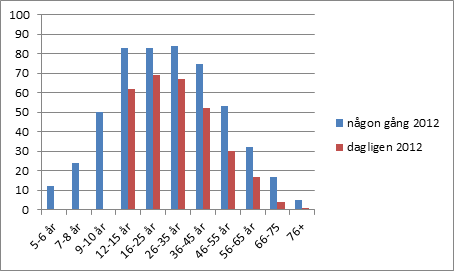
\includegraphics[scale=0.8]{pics/statistikalder.png}
    \caption{Andel procent av befolkningen som använder sig av mobilt internet, statistik visar att den stora målgruppen är mellan 12-45 år gamla (\cite[s. 24]{.se}).}
\end{figure}

\paragraph{Kontext}\mbox{}

Med kontext menas sidans typiska innehåll och huvudsyftet för webbsidan. Beroende på webbsidans kontext kan användarna finna det simplare att använda antingen desktop, mobilen eller den enhet närmast till hands. De vetenskapliga artiklar som har analyserats i litteraturstudien har alla gemensamt att mobilt internet används flitigt för:

\begin{itemize}
	\item{Sköta e-post}
	\item{Sociala nätverk}
	\item{Kolla nyheter, väder}
	\item{Söka information}
\end{itemize}
\bigskip
Andel procent av användarna skiljer sig beroende på artikel och statistik, då antalet användare för studierna har varit olika. Analysen visar ändå vad fokus läggs på när mobilt internet används. I Sverige uppskattas  50\% använda sig av mobilt internet för att sköta e-post, 43\% för socialt nätverk, 40\% för att kolla vädret, nyheter och 18\% för att söka fakta (\cite[s. 25]{.se}). I en annan studie där användningen av mobilt internet analyserades med hjälp av 109 deltagare visade den att 70\% av deltagarna använder mobilt internet för att kolla nyheter, väder och söka fakta, 13\% utav deltagarna använder mobilt internet för sociala nätverk och 17\% för att kolla på film och lyssna på musik(\cite{usageusability2}). I en liknande studie där 18 aktiva mobilanvändare studerades varje dag under en 4 veckors period, bestod den dagliga användningen av mobilt internet 27\% för sociala nätverk, 24\% för koll på nyheter och vädret, 18.8\% för email, 14.9\% för vanlig surf, 10\% för mobilsök och 5.1\% för kartor och navigation (\cite{mobilewebsearch}).

För desktop anses dessa fyra områden vara minst lika populära. I en studie som gjordes hos The Harris Polls Research (\cite{harrispoll}) samlades 2400 vuxna varav 991 mobilt internet användare för att se hur enheterna används i jämförelse beroende på kontext. I studien hamnade \textit{Sköta e-post, sociala nätverk och söka information} längst upp som de typer av hemsida vars desktopanvändare är ungefär lika stora om mobilanvändare.
\\
\begin{table}[H]
	\centering
	\begin{tabular}{|p{4cm}|p{4cm}|p{4cm}|}
	\hline
	~&Dator(desktop/laptop)&Mobil(Smartphone)\\ \hline
	Sköta E-post &90\%&72\%\\ \hline
	Sociala Nätverk&69\%&64\%\\ \hline
	Söka information&81\%&45\%\\ \hline
	Kolla nyheter, väder&44.2\%&52.1\%\\ \hline
	\end{tabular}
    \caption {Områden i webben där användarna utnyttjar både mobil och desktop.}
\end{table}

I studien ingick inte läsning av nyheter, men i Q1 Research report för nyhetsläsning (\cite{q1research}) visades det sig, med undantag från målgruppen 65 år uppåt, att majoriteten av läsarna(59\% till 77\% i varje målgrupp) använder både mobil och desktop för att läsa nyheter. Studien visar även att nyhetsläsare från mobilen numera är större än läsarna från desktop.

I The HarrisPole Research fanns även siffror för områden där användaren föredrar en enhet mer än den andra.

\begin{table}[H]
	\centering
	\begin{tabular}{|p{4cm}|p{4cm}|p{4cm}|}
	\hline
	~&Dator(desktop/laptop)&Mobil(Smartphone)\\ \hline
	Fylla enkäter &86\%&24\%\\ \hline
	Handla produkter&78\%&23\%\\ \hline
	Navigation/Kartor&56\%&73\%\\ \hline
	\end{tabular}
    \caption {Områden i webben där användarna föredrar en enhet mer än de andra.}
\end{table}

\paragraph{Miljö} \mbox{}

En användares miljö har förändras tack vare mobilens handburna storlek. Det har gjort att miljön inte är längre är den vanliga sederliga hemma eller på kontor, utan kan vara i vilket sammanhang som helst och även vart som helst. Ett vanligt antagande är att mobilen endast används vid rörliga situationer (\cite[s.12]{mobilefirstluke}). Vilket vetenskapliga artiklar och statistik visar tvärtemot (\cite{mobilewebsearch}, \cite{mobilefirstluke}).

Författaren av "\textit{mobile first"} hänvisar(\cite[s.12]{mobilefirstluke}) till en enkätundersökning vilket visar användningen av internet genom smartphones:
\begin{itemize}
	\item{84\% använder det hemma.}
	\item{80\% använder det under diversa dötid genom dagen.}
	\item{74\% använder det i kötid och i väntan på möten.}
	\item{69\% använder det under shopping.}
	\item{64\% använder det på jobbet.}
	\item{62\% använder det under TV tittande.}
	\item{47\% använder det under pendling.}
\end{itemize}
\bigskip

En stor andel av smartphonebärare använder sig av mobilt internet i hemmet, vilket styrks av fler vetenskapliga artiklar (\cite{mobilewebsearch}, \cite{mobilefirstluke}). Studierna pekar på bekvämligheten som existerar vid användande av mobilen istället för desktop. Mobilen tillåter 1 minuts intervaller för användning av internet vid brådskande tillfällen, vilket kan anses vara omständliga via desktop (\cite{mobilewebsearch}). I studien där 18 deltagare skulle föra dagböcker (\cite{mobilewebsearch}) under en period av 4 veckor var över 70\% av inläggen om aktiviteter gjorda vid ett stationärt perspektiv, det vill säga, antingen på jobbet eller i hemmet. Bara 17\% av inläggen handlade om aktiviteter som gjordes vid resor, utomhus eller vid pendling.
\\
\begin{itemize}
	\item{49,6\% av inläggen handlade om aktiviteter i hemmet.}
	\item{21,8\% av inläggen handlade om aktiviteter på jobbet/universitetet.}
	\item{11,4\% av inläggen handlade om aktiviteter inomhus.}
	\item{9,6\% av inläggen handlade om aktiviteter under pendling eller transit.}
	\item{7,2\% av inläggen handlade om aktiviteter utomhus.}
	\item{0,5\% av inläggen handlade om aktiviteter under resa utomlands.}
\end{itemize}
\bigskip

\subsection{Implementation}
\subsubsection{Prototyp}
Efter resultatet av litteraturstudien blev prototypen en nyhetssida. Grunden till valet gjordes med hänvisning till resultatet från litteraturstudien där statistik visar att andelen desktop- och mobilbesökare hos nyhetssidor är jämnt fördelat och även en av de största inom mobilt internet. För att skapa sidan gjordes en jämförelse mellan stora nyhetssidor så som \href{http://www.aftonbladet.se}{aftonbladet.se}, \href{http://www.metro.co.uk}{metro.co.uk}, \href{http://www.globalnews.ca}{globalnews.ca} och \href{http://www.time.com}{time.com}, för att upprätthålla typiska element som finns hos nyhetssidor. Allt som finns i ena vyn finns även i den andra.

\paragraph{Banner}\mbox{}

Banner visar tydligt vilken sidan man har kommit till. Beskriver namnet på sidan och en slogan som beskriver typen av webbsida. Både i mobilt och i desktop går dessa inte att undgå för att det skapar ett igenkännande hos användaren. Däremot är bannern mindre på mobilsidan i förhållande till artiklarna tillskillnad från desktopvyn(\textit{figur 6}), för att undvika att bannern ta för stor plats på mobilskärmen(\textit{figur 7}).
\\
\begin{figure}[H]
\centerline{%
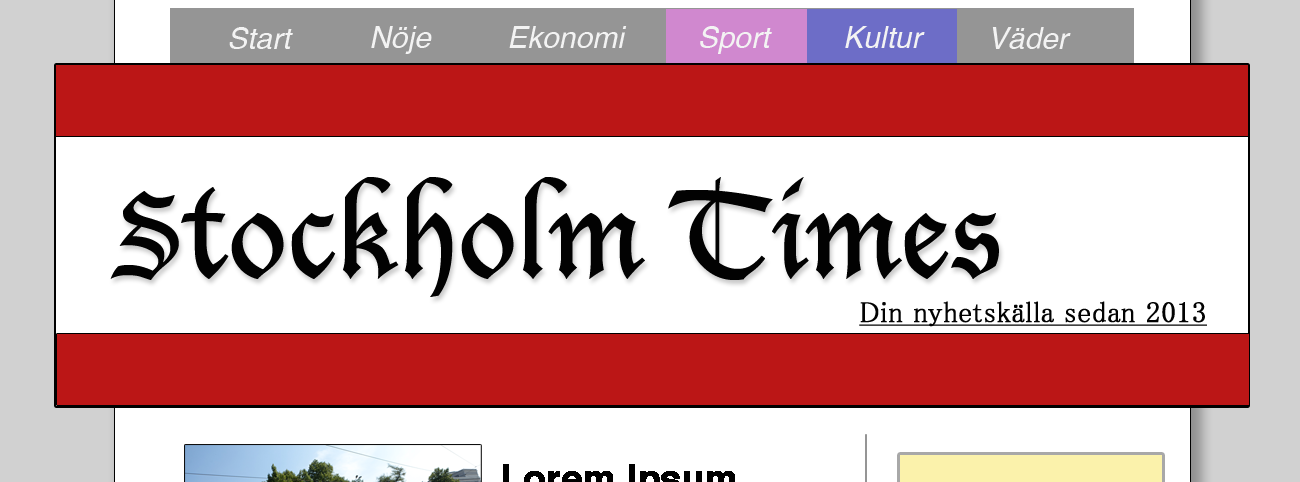
\includegraphics[scale=0.258]{pics/bannerdesktop.png}\hspace{2em}%

\includegraphics[scale=0.40]{pics/bannermobil.png}%
}
\vspace{0.3cm}
\hspace{0.15cm}Figur 6: Banner för desktopvyn.\hspace{4.4cm} Figur 7: Banner för mobilvyn.

\end{figure}

\paragraph{Menyer}\mbox{}

Nyhetssidorna som användes som referens för prototypen hade alla minst tre olika sorters menyer. En huvudmeny, en mindre meny bestående av typiska ”skapa konto, logga in” länkar(\textit{figur 8}), samt en nedre meny längst ner på sidan med diverse länkar(\textit{figur 10}). I mobilvyn behölls nedersta menyn i en ihopsamlad version och de två översta sattes ihop och gömdes under en menyknapp för att spara plats på mobilskärmen(\textit{figur 9}).
\\

\begin{figure}[H]
\centerline{%
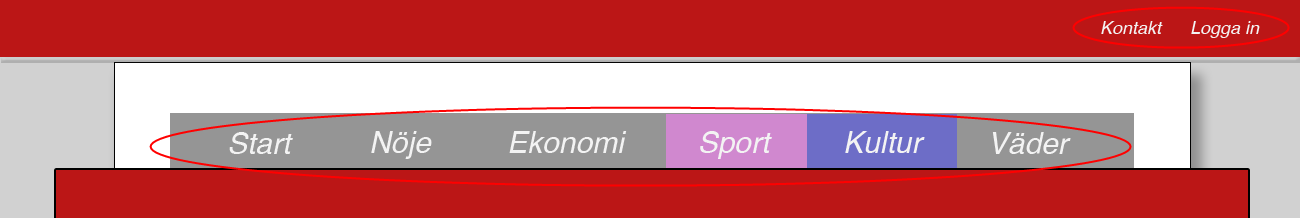
\includegraphics[scale=0.4]{pics/menydesktop.png}\\
}
\end{figure}
\hspace{0.5cm}Figur 8: Huvudmenyn i desktopvy.

\begin{figure}[H]
\centerline{%

\includegraphics[scale=0.6]{pics/menymobil.png}\hspace{2em}%
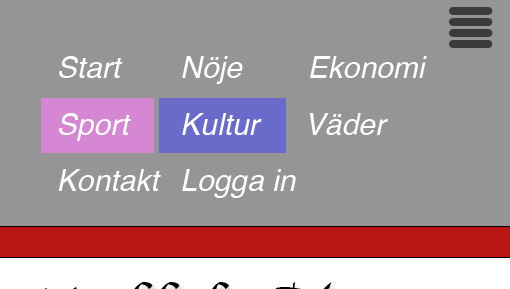
\includegraphics[scale=0.35]{pics/menymobilopen.png}%
}
\end{figure}
\hspace{0.5cm}Figur 9: Huvudmenyn i mobilvyn.

\begin{figure}[H]
\centerline{%
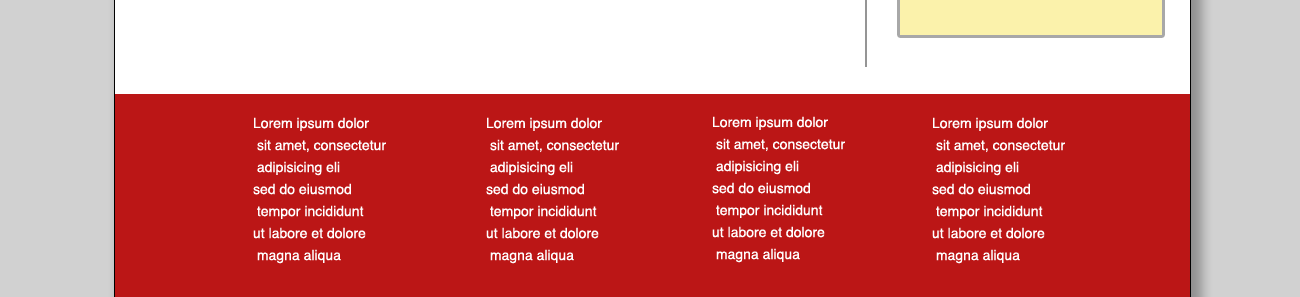
\includegraphics[scale=0.237]{pics/menydesktopbot.png}\hspace{2em}%
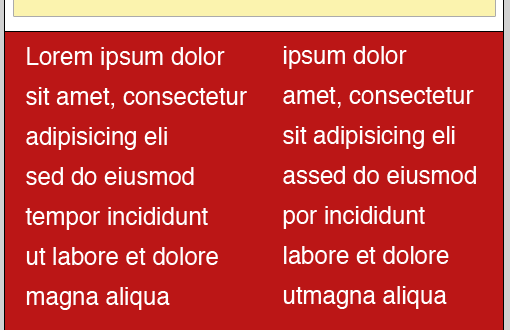
\includegraphics[scale=0.35]{pics/menymobilbot.png}%
}
\end{figure}
\hspace{0.5cm}Figur 10: Nedremenyn i desktopvyn och mobilvyn.
\newpage
\paragraph{Artiklar och Annonser}\mbox{}

Artiklarna och annonserna prioriterades ungefär lika högt i desktopvyn(\textit{figur 11}) för att annonser anses vara en viktig faktor till nyhetssidors intäkter. Dessvärre inte samma prioritering i mobilläge, då ytan är mindre och artiklarna är huvudelementen på nyhetssidan. Därför hamnade annonserna i mobilvyn efter artiklarna(\textit{figur 12}). Artiklarna har alla samma storlek men skiftar i plats på bild och text för att skapa en mer levande känsla hos webbsidan. Annonsernas design härstammar från \href{www.aftonbladet.se}{aftonbladet.se}, där färgen på bakgrunden samt texten får läsaren att förstå att det är annonser. 
\\

\begin{figure}[H]
\centerline{%
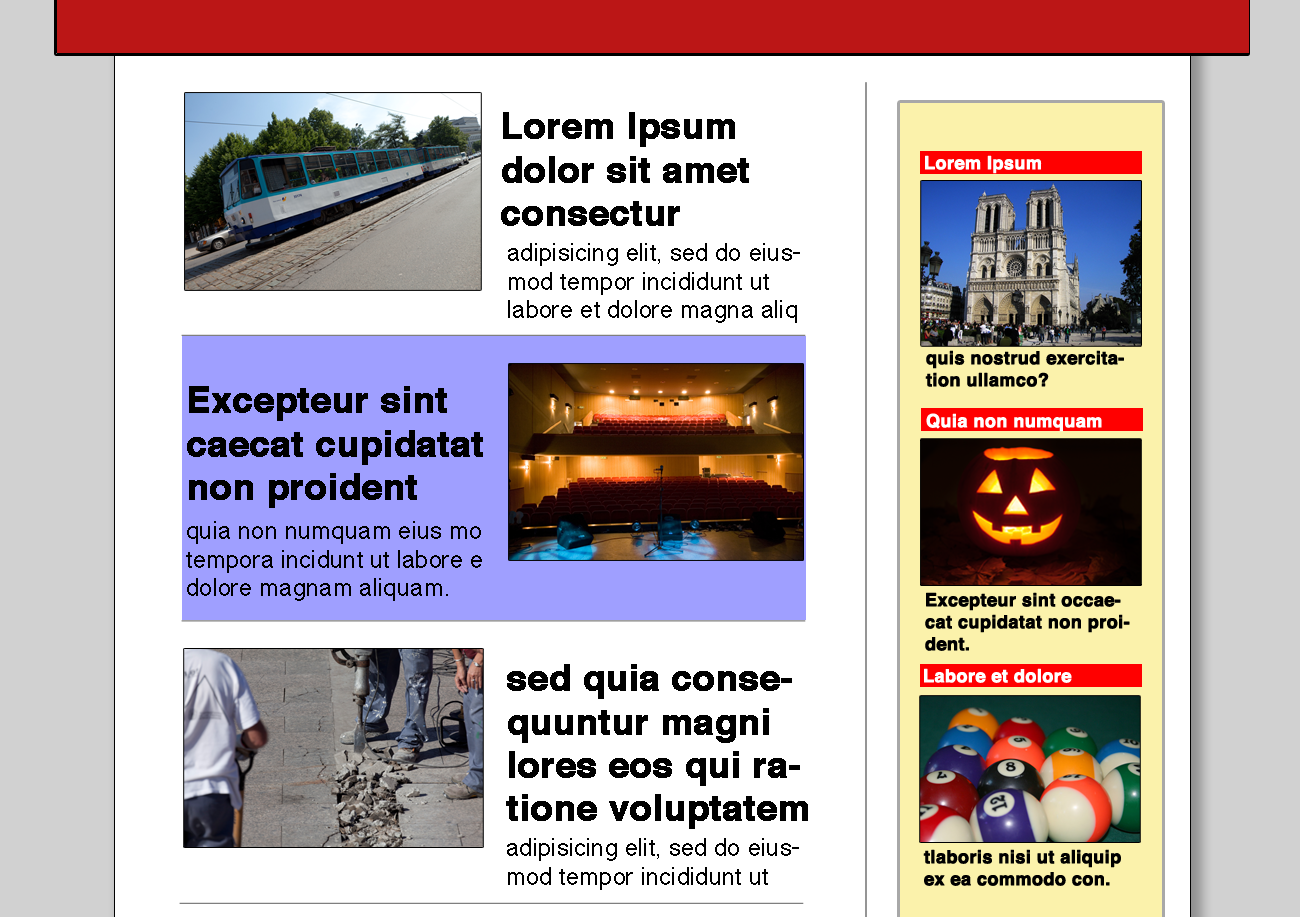
\includegraphics[scale=0.3]{pics/artikelannonsdesktop.png}
}
\end{figure}
\hspace{0.5cm}Figur 11: Artiklar och annonser i desktopvyn.
\\
\begin{figure}[H]
\centerline{%
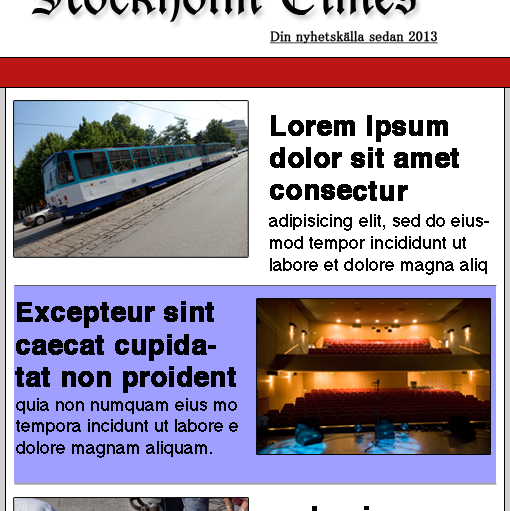
\includegraphics[scale=0.35]{pics/artikelmobil.png}\hspace{2em}%
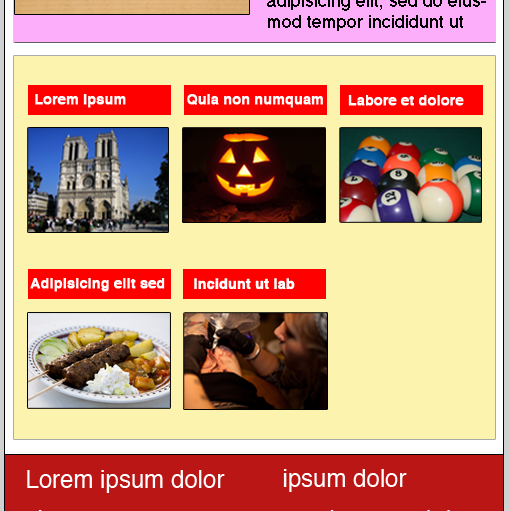
\includegraphics[scale=0.35]{pics/annonsmobil.png}%
}
\end{figure}
\hspace{0.5cm}Figur 12: Artiklar och annonser i mobilvyn.

\paragraph{Färgmarkeringar}\mbox{}

Färgmarkeringen görs i webbsidan för att markera olika typer av artiklar. På nyhetssidor görs detta för att markera artiklar som tillhör en annan sektion av tidningen, t.ex sport, ekonomi, kultur osv. I prototypen markeras sport och kultur med en rosa och blå färg vilken även blir färgen för respektive länk(\textit{figur 13}).
\\

\begin{figure}[H]
\centerline{%
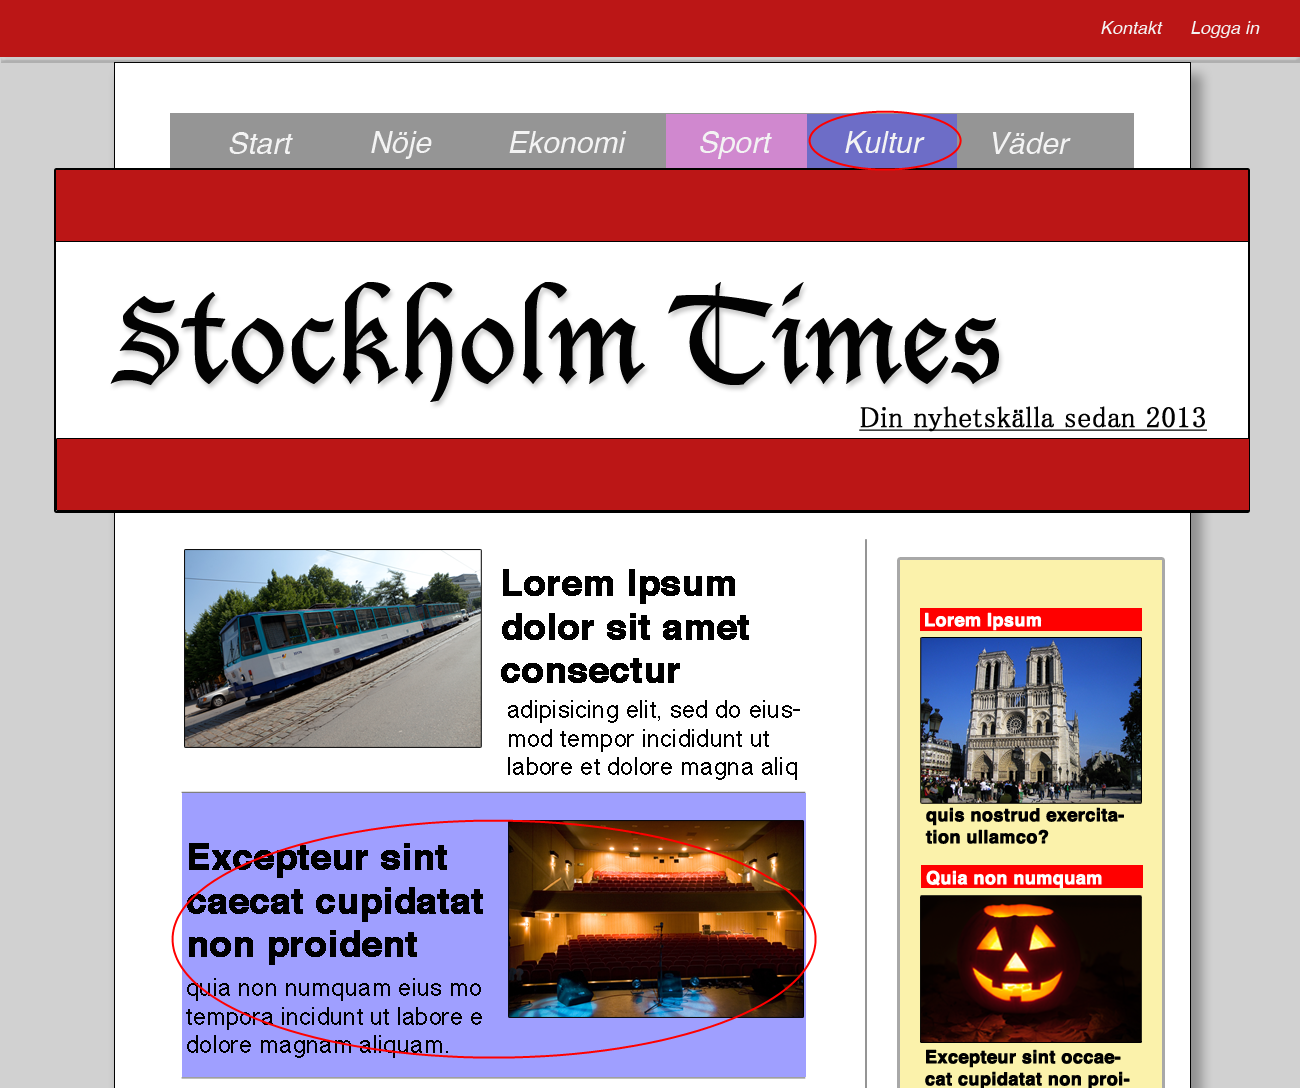
\includegraphics[scale=0.25]{pics/fargdesktop.png}\hspace{2em}%
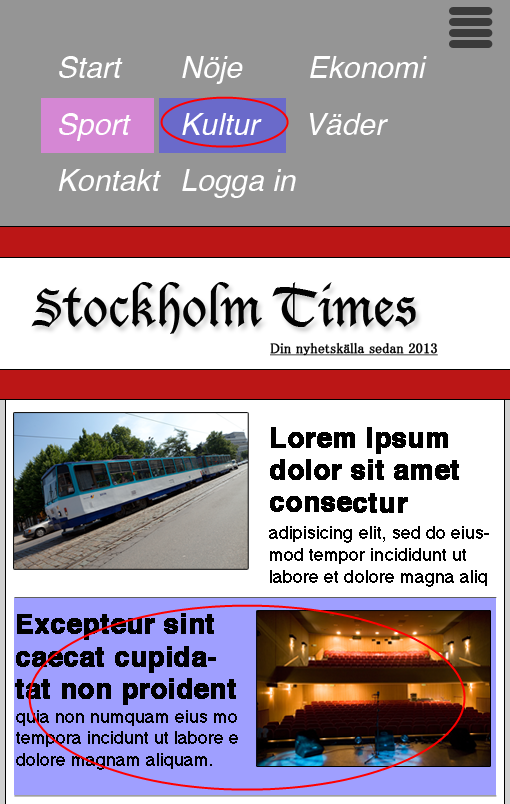
\includegraphics[scale=0.3]{pics/fargmobil.png}%
}
\end{figure}
\hspace{0.5cm}Figur 13: Blå färgmarkering för kultursektionen.


\subsubsection{Responstid}

Nedan visas tre olika hämtningar av bägge webbsidor, både i desktopmiljö samt mobilmiljö. Värdena som har antecknats är responstiden för hämtning av HTML-filen samt CSS-filen. Sambandet mellan de olika hämtningar visar att mobilvyn laddas snabbare i mobile-first och desktopvyn laddas snabbare i desktop-first.

\newpage
\textbf{Hämtning 1}

\begin{table}[H]
	\centering
	\begin{tabular}{|p{2.5cm}|p{2.7cm}|p{2.4cm}|p{3.1cm}|p{2.8cm}|}
	\hline
	~&\textbf{.html mobilvy}&\textbf{.css mobilvy}&\textbf{.html desktopvy}&\textbf{.css desktopvy}\\ \hline
	\textbf{Desktop-first}&73ms&36ms&36ms&21ms\\ \hline
	\textbf{Mobile-first}&36ms&19ms&39ms&23ms \\ \hline
	~&~&~ &~&~\\ \hline
	\end{tabular}
    \caption {Värden från första hämtningen av prototypsidan. Tabellen visar tydligt snabbare responstid för mobilvyn med mobile-first och snabbare responstid för desktopvyn med desktop-first. Anmärkningsvärt är värderna för laddningen av css-filen i mobilvyn, där det tar mobile-first 19ms, men desktop-first 36ms.}
\end{table}

\textbf{Hämtning 2}

\begin{table}[H]
	\centering
	\begin{tabular}{|p{2.5cm}|p{2.7cm}|p{2.4cm}|p{3.1cm}|p{2.8cm}|}
	\hline
	~&\textbf{.html mobilvy}&\textbf{.css mobilvy}&\textbf{.html desktopvy}&\textbf{.css desktopvy}\\ \hline
	\textbf{Desktop-first}&19ms&22ms&46ms&20ms\\ \hline
	\textbf{Mobile-first}&33ms&20ms&22ms&22ms \\ \hline
	~&~&~ &~&~\\ \hline
	\end{tabular}
    \caption {Värden från andra hämtningen av prototypsidan. Ungefär samma resultat som tabell 5, men med mindre skillnad mellan responstiderna. Tabellen visar ändå en snabbare hämtning av css-filen för mobile-first i mobilvyn respektive desktop-first i desktopvyn.}
\end{table}

\textbf{Hämtning 3}

\begin{table}[H]
	\centering
	\begin{tabular}{|p{2.5cm}|p{2.7cm}|p{2.4cm}|p{3.1cm}|p{2.8cm}|}
	\hline
	~&\textbf{.html mobilvy}&\textbf{.css mobilvy}&\textbf{.html desktopvy}&\textbf{.css desktopvy}\\ \hline
	\textbf{Desktop-first}&37ms&22ms&20ms&19ms\\ \hline
	\textbf{Mobile-first}&16ms&18ms&32ms&20ms \\ \hline
	~&~&~ &~&~\\ \hline
	\end{tabular}
    \caption {Värden för tredje hämtningen av prototypsidan. Hämtning av css i mobilvyn är snabbare för mobile-first med 4ms skillnad, däremot är css hämtningen i desktopvyn snabbare för desktop-first, men med bara 1ms i skillnad.}
\end{table}

Hämtningarna visar tydligt att css-filen laddas snabbare för mobile-first i mobilvyn och snabbare för desktop-first i desktopvyn. Gällande hämtning av html-filen följer det samma mönster förutom i en av hämtningarna(\textit{tabell 6}). Där är resultatet tvärtom från resultatet i tabell 5 och 6. Alla hämtningar har gjorts från en stationär dator med en emulator som renderar om webbläsarens storlek för att passa vald enhet. Utförligare analys angående responstiden diskuteras i diskussionavsnittet.

\subsubsection{Kodstorlek}

Tabellen visar storleken på css-filen i både antal rader och filstorlek. Den visar att CSSen för mobil-first är större än CSSen för desktop-first i filstorlek. Däremot har den i desktop-first fler rader än den i mobile-first. I mobile-first är uppdelningen i CSSen mellan rader i grundkod och rader i media queries, 193 mot 180. I den för desktop-first består den större delen av rader i grundkoden, där är uppdelningen 221 mot 160.

\begin{table}[H]
	\centering
	\begin{tabular}{|p{6cm}|p{2.7cm}|p{2.4cm}|}
	\hline
	\textbf{main.css}&\textbf{Desktop-first}&\textbf{Mobile-first}\\ \hline
	\textbf{Antal rader i grundkod}&221st&193st\\ \hline
	\textbf{Antal rader i media queries}&160st&180st\\ \hline
	\textbf{Totalt antal rader}&381st&373st\\ \hline
	\textbf{Filstorlek}&5.2kb&5.6kb\\ \hline
	\end{tabular}
    \caption {Värden från main.css.}
\end{table}

\subsubsection{Implementeringstid}

Implementeringstiden redovisas utifrån dagboken som skrevs under implementationsfasen. Resultatet visar skillnaden mellan implementeringstiden för grundsidan och tiden som krävdes för att göra webbsidan responsiv med hjälp av media queries. I mobile-first tog grundsidan mindre tid att implementera än att göra webbsidan responsiv. I desktop-first tog det däremot längre tid att implementera grundsidan. Desktop-first tog totalt längre tid att implementera än mobile-first. Ta i beaktande att implementeringen gjordes av en junior inom området gränssnittsutveckling, samt att desktop-first implementerades före mobile-first.

\begin{table}[H]
	\centering
	\begin{tabular}{|p{6cm}|p{2.7cm}|p{2.4cm}|}
	\hline
	~&\textbf{Desktop-first}&\textbf{Mobile-first}\\ \hline
	\textbf{Tid för grundsidan}&14.5h&6.5h\\ \hline
	\textbf{Tid för responsive}&7.5h&10h\\ \hline
	\textbf{Totalt tid}&22h&16.5h\\ \hline
	\end{tabular}
    \caption {Värden på implementationstid, hämtade från dagboken.}
\end{table}

\subsubsection{Kommentarer från dagboken}

\textbf{Desktop-first}
\\\\
\textit{”Mycket småpill i början, många element att finslipa, göra fina och sättas på plats.”}\\\\
\textit{”Oerhört lätt att göras till responsive så länge man har använt sig av fluid grid och fluid layout från början. Allt renderas av sig självt och så fort det ser konstigt ut, modifieras CSSen i media queries.”}\\\\
\textit{”Lång tid i början, i jämförelse med responsive delen. Förvånad över att responsivedelen gick så smidigt. Endast lite småpill lite här och där för att fixa storleken på text, margins och paddings. Det mesta hade fixats under desktoputseendet.”}\\\\
\textit{”Inte så många media queries, sidan ser bra ut mellan media queries. Mycket kod i grunden som är avsedd för desktop, inte lika mycket i media queries.”}\\\\
\textbf{Sammanfattning:} Skapandet av grundsidan var det som tog mest tid, då det innebar många element att designa och positionera på rätt plats. Den responsiva delen gick smidigt till då media queries, fluid grid och fluid images enkelt renderar om elementen till att vara mindre och positioneras under varandra i en kolumn anpassad till mobilskärmen.
\vspace{0.735cm}
\\
\textbf{Mobile-first}
\\\\
\textit{”Enkelt sätt att påbörja webbsidan, följer skissen uppifrån neråt, går inte att tappat bort sig åt kanterna, utan elementen är så pass små att det känns som att de finns i en smal led att följa.”}\\\\
\textit{”Behövs mycket småpill mellan media queries. Media queries kommer i början hyfsat tät inpå varandra enbart för att fixa små fel som margins och padding så att elementen håller sig på ett och samma ställe. Samt för förstoring av text, som är väldigt liten i början och måste förstoras i media queries då det inte kan använda sig av fluid grid.”}\\\\
\textit{”Gäller att hitta en struktur redan från början mellan skisserna. Det blir några refaktoreringar för att få webbsidan, då bredden är 768px, att se perfekt ut, eftersom mycket ändras just under den vyn.”}\\\\
\textit{”Från 768px till desktop-size gick väldigt smidigt.”}\\\\
\textit{”Väldigt lätt i början, enkel struktur att lägga upp för mobilen. Responsivt höll det till 480px, till och med 768px var det mycket att fixa med hjälp av media queries, då många element går från att vara under varandra till att vara bredvid varandra.”}\\\\
\textit{”Viktigt att planera och lägga en struktur på hur den ska övergå till desktop. Mycket kod i media queries sektionen, lite kod i grunden för mobilvyn.  Ser bra ut mellan mobilvyn och desktopvyn.”}\\\\
\textbf{Sammanfattning:} Skapandet av grundsidan gick fort, var stabil och väl strukturerad. Däremot krävdes det fler media queries i början av den responsiva delen då mycket förändras tidigt. Det är viktigt att lägga upp en bra planering till hur webbsidan skall övergå till desktopvyn, då element övergår till att positioneras utspritt över webbplatsen.



\section{Diskussion}
\subsection{Mobile- vs Desktop-first}
Mobile-first kontra desktop-first har varit den stora frågan i arbetet, efter litteraturstudien och implementationen har tydligheten i metodernas områden blivit allt klarare och har under arbetets gång även blivit mer populärt bland bloggar. I resultatet för litteraturstudien samlades synpunkter från 13 olika källor, vilka inläggsdatum för de flesta inte är mer än ett år gamla. Av dessa källor är det 11 som förespråkar för mobile-first, en som föredrar desktop-first och en som anser att tekniken är för ny för att förorda(inlägg från 2011). Implementationsfasen bekräftar mycket av det som har sagts i litteraturstudien, både till fördel för desktop-first och mobile-first. Men i slutändan har implementationen utav webbsidorna visat sig vara kodmässigt relativt lika, mobile-first använder sig utav min-width, medan desktop-first använder sig utav max-width, mobile-first ser till att rendera om elementen när skärmen blir större och desktop-first när skärmen blir mindre.
Mycket fokus har lagts på metoderna för sig, när ett större problem visar sig vara skillnaden mellan mobilen och desktopens kapacitet. Mobiler har sämre prestanda, mindre skärm och bandbreddsbegränsningar, vilket inte existerar i samma utsträckning hos datorer. Dagens mobiler har kommit långt i utvecklingen men kan inte mäta sig med datorn.
Det visade sig att arbetet kom att handla om vilken metod \textbf{passar} bäst i dagens teknik och inte vilken metod som \textbf{är} bäst. Dagens internet användning utgörs mestadels ifrån mobiler och datorer, där mobilen är de enhet som presterar sämre. 

Mobile-first tar sig an problem som mobilen har och ser till att det utför det simplaste och läser in så lite som möjligt av webbsidan, med andra ord endast den kod som är avsedd för mobilen. Det finns det ingen metod som tillför samma sorts fördel för båda enheter, utan mobile-first kommer att behöva läsa in mer när webbsidan ses ifrån skrivbordskärmen då den läser både allt för mobil och även det som skall ändras för desktop. Desktop-first läser in det nödvändigaste för skrivbordskärmen, men när webbsidan ses ifrån en mobil, kommer den läsa in allt för desktop och sedan allt som den behöver ändra för att webbsidan skall passa mobilen. Detta betyder att mobil-first kommer se till att mindre läses in för den enhet vars prestanda är låg och mer läses från den enhet vars prestanda är hög och har kapaciteten att hantera det.

I litteraturstudien nämndes att mobile-first bidrar till en robust grund för komplikationer som prestanda, design, och prioritering av element. Prestanda visas nedan i diskussionen genom responstid och kodalanys, men design och prioritering är lite svårare att visa. I arbetet designades både mobilvyn och desktopvyn samtidigt, sida vid sida och vid ett tidigt skede bestämdes att båda vyerna skulle innehålla samma funktioner. Med anledning att användare skall ha samma möjligheter vare sig enhet webbsidan ses ifrån. I litteraturstudien ses detta som ett tillvägagångsätt som existerar i mobile-first där meningen istället översätts till \textit{”Får inte någonting plats i mobilvyn, så ska den inte heller få finnas i desktopvyn”.} Detta används för att undvika att funktionalitet endast finns på en av enheterna. Anledningen till att det är ett mobile-first princip är för att det är hos mobilen då element kan ha svårigheter att få plats, på grund av den begränsade skärmstorleken. Prioriteringen i mobilvyn sker då vid ett tidigt skede och allt som får plats i mobilskärmen kommer att få plats på en större skärm. I desktop-first gäller inte samma princip då element i en större skärm inte alltid får plats i en mindre yta. Det leder till att prioriteringen kommer i efterhand, och sker endast för mobilvyn, vilket kommer sakna funktionalitet som finns för desktopvyn och där mobilvyn istället blir en komplement till desktopsidan. En användare som tidigare har varit på desktopsidan kommer att sakna dessa funktioner i mobilvyn och då har webbsidan plötsligt tappat sitt syfte för en mobilanvändare. 
I arbetet dök aldrig problemet upp för att principen \textit{"om inte ett element fick plats i mobil designen så fick den inte finnas i desktopdesignen} följdes från start.

Respons tid, kodanalys, implementerings tid och skärmstorlek är en av de större faktorer som stärker de påståenden taget från litteraturstudien, nedan beskrivs och analyseras dessa i synnerhet till de praktiska och teoretiska tillvägagångssätt.

\subsubsection{Responstid}
Responstid är den tid det tar mellan att en begäran har lagts, till dess att begäran har utförts, det vill säga i webbsammanhang den tid det där att hämta och visa elementen på webbsidan. De tre hämtningar visar klart att när webbsidan ses utifrån ett mobilperspektiv hämtas css-värden för att rita ut elementen snabbare med mobile-first än med desktop-first\textit{(tabell 5 ,6 ,7)}. När webbsidan ses utifrån ett desktopperspektiv hämtas css värderna snabbare med desktop-first än med mobile-first. Det vill säga, mobil-first ger bra siffror för hämtningar från mobilvyn och desktop-first bra siffror för hämtningar från desktopvyn, båda lika bra i sitt område om man skulle vilja jämföra metoderna strikt gentemot varandra. Att metoderna är bäst för var sin vy är förståeligt eftersom mobile-first i mobilvyn endast läser grundkoden utan att behöva ändra något värde i media queries, desktop fungerar bra i desktopvyn för att den endast läser grundkoden för desktopvyn. Men som tidigare poängterats i diskussionen handlar det inte om metoderna var för sig utan enheterna webbsidan ses från, där responstiderna för mobile-first gynnar den enhet med sämre prestanda vilket desktop-first inte gör. Båda responstiderna för mobil-first och desktop-first är hämtade från en dator där en emulator som minskar webbläsaren till en iphones storlek har använts. Skillnaden mellan responstiderna är väldigt låga, ibland endast 2 millisekunder, för att prestandan och bandbredden som har använts för att hämta webbsidorna är ifrån en dator. 

Ändå visar responstiden på en skillnad, men i verkligheten är inte omständigheterna likadana som i testfallen. En desktop-first sida som ses i mobilvyn tog enligt en av hämtningar 36ms och desktyopvyn 21ms. 21ms är relativt snabbt, vilket även 36ms är. När desktop-first sidan ses på en skrivbordskärm kommer hämtningen av css-en ta ungefär 21ms, men när vi ser en desktop-first sida på mobilen kommer den inte nödvändigtvis att ta 36ms som det står i tabellen\textit{(tabell 5)}. Detta för att mobilen inte har samma prestanda och bredbandsmöjligheter som datorn som användes för hämtningar. Skillnaden mellan desktop-first och mobile-first blir inte längre 2ms, utan måste multipliceras med faktorerna, sämre prestanda och bredband. Vilket leder till att skillnaden blir mellan metoderna blir oerhört större än vad som har visats i tabellen för hämtningarna av css-filen. Mobile-first visar genom tabellerna\textit{(tabell 5 ,6 ,7)} att enheter där webbsidan ses i mobilvy inte behöva ladda mer än vad som behövs för att visa webbsidan och låter de enheter med bättre omständigheter ta på sig att hämta mer än nödvändigt.

Förutom att hämtningarna är gjorda med en dator så måste prototypen has i åtanke då den egentligen bara speglar skalet av en fulländad webbsida. Det vill säga att hämtningarna som görs är för en webbsida som är relativt liten i jämförelse med en normal webbsida. Återigen är dessa 2ms i skillnad mellan metoderna i en hämtning av mobilvyn små i jämförelse med vad skillnaden skulle vara om prototypen hade varit för ett större projekt.

Resultat av responstiden visar tydligt de punkter som diskuterats i litteraturstudien. Mobile-first ger en robust webbsida för mobilen som fokuserar i första hand på situationer hos användaren där snabb respons krävs. Tack vare prestandan hos dagens datorer utelämnar inte mobile-first desktop, utan låter den snarare ta hand om den större lasten, vilken den har kapacitet för.

\subsubsection{Kodanalys}
\paragraph{Storlek}\mbox{}

Kodstorleken spelar en stor roll till resultatet av responstiden, beroende på metod läser webbsidorna olika mycket av css-koden för att renderera sidan beroende på webbläsarens bredd. Main.css består utav grundkoden, där elementen definieras och får de egenskaper för att ritas ut på webbläsaren och media queries koden, där dessa värden ändras för att anpassas efter webbläsarfönstret. Totalt antal rader är ungefär samma mellan desktop-first och mobile-first\textit{(tabell 8)}. Det som skiljer sig är antal rader av kod som metoderna har i grunden och i media queries. I mobile-first är grundkoden avsedd för mobilen, vilket betyder att den endast läser grundkoden när webbsidan ses i mobilvy, vilket är 193 rader. I desktop-first är grundkoden avsedd för desktop och läser endast in den vid desktopvy, vilket består av 221 rader. Om det kommer sig att webbsidan ses utifrån den vy vars metoden inte är avsedd för, betyder det att den måste läsa in all grundkod och sedan koden från media queries för att ändra egenskaperna för varje element. I desktop-first måste mobilwebbläsaren läsa totalt 381 rader för att kunna visa webbsidan, i mobile-first måste desktopwebbläsaren läsa totalt 374 rader för att kunna visa webbsidan. Båda metoder har sina fördelar och inriktar sig för att fungera bäst för var sin enhet. Men återigen måste enheterna has i åtanke. Mobilen har inte samma prestanda som en dator, antingen läses det in få rader kod i mobilen och många rader kod i desktop, eller många rader i mobilen och få rader i desktop. Det visar fördelarna som diskuterades i litteraturstudien, vilka innebär att låta mobilen läsa in så lite som möjligt på grund av prestandaskäl och datorn mer än nödvändigt då den har kapaciteten att kunna hantera det. 

\paragraph{komplexitet}\mbox{}

Förutom olika mycket kod i media queries, skiljer sig metodernas main.css till att få mobile-first agera som ett mer naturligt sätt att implementera. I Mobile-first är grundkoden avsedd för mobilen där element ligger i en kolumn under varandra. Eftersom det är standard att element visas under varandra behövs ingen kod för detta, utan kod läggs istället till i media queries när webbsidan börjar övergå till desktop och element skall visas vid sidan om varandra. I desktop-first måste elementen redan från början definieras så att de skall ligga bredvid varandra då detta inte är standard. När webbsidan börjar övergå till mobilläge och webbläsaren blir mindre, måste i media queries se till att det blir ogjort så att elementen hamnar under varandra, i en kolumn. Med andra ord kräver detta en rad kod i mobil-first som ändrar elementens position när den syns i desktop(\textit{figur 14}), men två rader kod i desktop-first, en som ändrar elementens position från början och en som ser till att det återgår till standard när sidan syns i mobilen(\textit{figur 15}). Det är endast fåtal element i protoypen där detta förekommer, men det tyder på att fallet existerar fler gånger på större webbsidor, speciellt nyhetssidor, där många element går från att vara vid sidan om varandra till att vara under varandra i en kolumn. Det medför att mobilsida blir ett naturligt sätt att påbörja en implementation av en responsiv webbplats, då det börjas från standard. 

\setcounter{figure}{13}
\begin{figure}[H]
  \begin{subfigure}[b]{.5\linewidth }

    \begin{lstlisting}
     .articles{
	color: white;
	widht: 200px;
	height:200px;
      }

    @media (min-width: 768px){
	float:left;
    }
 & &
    \end{lstlisting}
    \caption{Mobile-first}
    \end{subfigure}
    \begin{subfigure}[b]{.5\linewidth}
	\begin{lstlisting}
     .articles{
	float:left;
	color: white;
	widht: 200px;
	height:200px;
      }

     @media (max-width: 768px){
	float: none;  
     }
	\end{lstlisting}
    \caption{Desktop-first}
  \end{subfigure}
  \caption{I Desktop-first(b) måste elementet först definieras så att de ligger vid sidan om varandra, sedan med media queries tas detta bort när det går över till mobilvyn. I Mobile-first(a) är det standard och inget behöver definieras förens webbsidan övergår till desktopvy, då sätts elementen vid sidan om varandra.}
\end{figure}
\newpage
\subsubsection{Implementeringstid}
Implementeringstiden för webbsidorna skiljer sig med ungefär med 5 timmar, mobil-first tog totalt 16,5 timmar och desktop-first 22h. Det är svårt att dra slutsatsen att mobile-first tar mindre tid att implementera än desktop-first, på grund av att: 1. Desktop-first implementerades före mobile-first, för en junior gränssnittsutvecklare, kan desktop-first implementeringen varit en bra uppvärmning, 2. För att erfarenheten utav utvecklaren inte är tillräckligt stor, vilket kan medföra inlärning inräknat i tiden. En teori kan ändå skapas utav kommentarerna ur dagboken och även tiden som redovisades under implementationsfasen

Grundsidan för desktop-first tog längst tid att implementera, vilket enligt dagboken krävde många element att dekoreras och positioneras utspritt på en stor yta. Saknas erfarenhet inom området, kan det vara svårt att finna en struktur på hur en webbsida skall formas. Grundsidan för mobile-first tog minst tid, vilket i dagboken beskrivs som ett enkelt sätt att forma en webbsida på. Innehållet är i en kolumn där element implementeras uppifrån neråt utan att kunna tappa bort sig åt sidorna eller ändra något som påverkar andra element. Att göra webbsidan responsiv tog mindre tid för desktop-first än mobile-first. I desktop-first har elementen dekorerats och lagts ut på rätt plats, det enda som behövs göras är att minska elementen och samla ihop dessa till en kolumn, vilket fluid grid, fluid images och media queries tar hand om utan att gränssnittsutvecklaren behöver justera för mycket. I mobile-first börjar elementen i en kolumn, det som skall göras är att låta fluid grid, fluid images göra så att dessa förstoras. I mobile-first krävs det däremot fler justeringar i media queries då elementen skall positioneras till sina utspridda platser på desktopvyn istället för en kolumn där elementen finns under varandra. Det kan vara anledningen till att responsivdelen för mobile-first tog längre tid än responsivdelen i desktop-first.

Mobile-first har fördelen att grundsidan implementeras på ett simplare sätt än i desktop-first. Istället för att rita ut alla element utspridda på en sida, dekoreras detta i en kolumn och låter den responsiva delen ta hand så att elementen hamnar på rätt plats i desktopvyn, med ett antal justeringar med media queries(\textit{figur 15}). I desktop-first, sprids och dekoreras elementen för att sen låta den responsiv delen samla in dessa i en kolumn, men då har redan mycket tid lagts åt att rita och positionera ut elementen i desktopvyn(\textit{figur 16}). Teoring säger att mobile-first är ett mer effektivt tillvägagångsätt, men att om behovet istället är en snabb lösning till att göra en existerande webbsida responsivt, finns fördelen tidsmässigt hos desktop-first då grunden redan är lagd.
\\
\begin{figure}[H]
\centerline{%
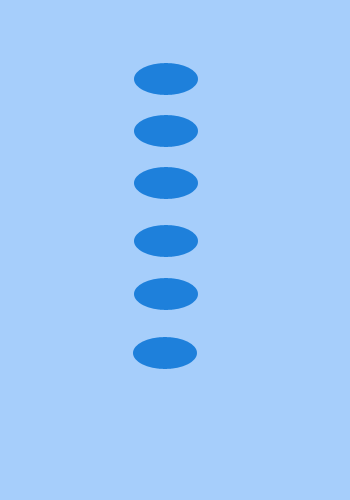
\includegraphics[scale=0.27]{pics/mobiledots.png}\hspace{2em}%
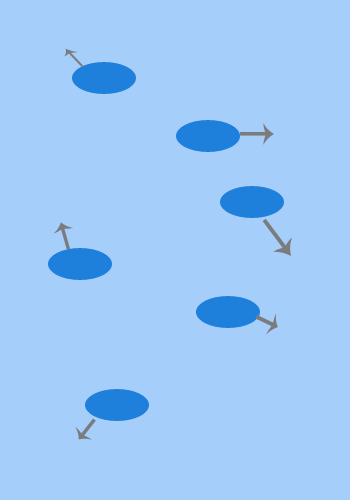
\includegraphics[scale=0.27]{pics/responsiv.png}\hspace{2em}%

\includegraphics[scale=0.27]{pics/desktop.png}%
}
\hspace{2cm}(a) Mobilvyn\hspace{2.3cm}(b)Responsiv\hspace{2.1cm}(c) Desktopvyn
\\\\
\hspace{0.15cm}Figur 15: Responsiv i Mobile-first, elementen börjar designas och placeras i en kolumn på skärmen, responsive ser till att med en del justeringar placera dessa rätt i desktopvyn.
\end{figure}

\begin{figure}[H]
\centerline{%

\includegraphics[scale=0.27]{pics/desktop.png}\hspace{2em}%

\includegraphics[scale=0.27]{pics/desktopresp.png}\hspace{2em}%
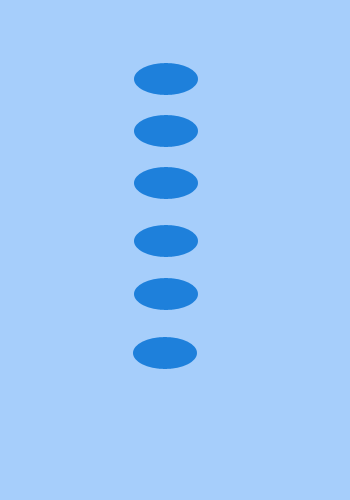
\includegraphics[scale=0.27]{pics/mobiledots.png}%
}
\hspace{1.7cm}(a) Desktopvyn\hspace{2.3cm}(b)Responsiv\hspace{2.1cm}(c) Mobilvyn
\\\\
\hspace{0.15cm}Figur 16: Responsiv i Desktop-first, elementen måste designas och placeras rätt på skärmen, responsiv ser till att de samlas en kolumn för mobilvyn.
\end{figure}


\subsubsection{Skärmstorlek}
Storleken på mobilskärmen har i litteraturstudien setts som ett hinder, en barriär som kräver fokus där en design tas fram efter en prioritering av de nödvändigaste funktionerna. Under implementeringen var skärmstorleken en lättnad, en kompakt design som ledde till struktur i arbetssättet. Prototypen av webbsidan var en förenklad version utav riktiga nyhetssidor, därför är det inte lika lätt att förstå sig på prioriteringssvårigheten som kan uppkomma på större webbsidor.

Prototypen innehöll inte lika många element som en verklig nyhetssida, vilket gör det svårt att relatera till prioriteringssvårigheten som webbutvecklare i litteraturstudien har beskrivit. I desktop-first är skärmstorleken stor, där prioritering av funktionalitet inte har samma betydelse som i mobile-first, då det mesta får plats. Däremot visar detta återigen risken att för att mobilvyn istället blir en förenklad och nerskalad version utav desktop-sidan. Skärmstorleken bör ses som ett hjälpmedel istället för ett hinder. Ett hjälpmedel för utvecklaren och interaktionsdesignen som försäkrar att funktionalitet inte försvinner mellan vyer och samtidigt skapar en bra grund, för både arbetssätt och användbarhet. Användbarhet har eskalerat inom webbutveckling, vilket av egen erfarenhet anses vara högt prioriterande. I litteraturstudien delas denna åsikt med härledning till att webben börja ses i ett annat perspektiv, där funktionalitet och användbarhet uppskattas mer än mäktig design som kan kräva mycket prestanda, speciellt för en mobil. Desktop-first är inte nödvändigtvis ett hinder för att skapa en användaranpassas webbsida, men mobil-first är en försäkran att detta upprätthålls, tack vare mobilens kompakta skärmstorlek som kräver fokus på innehåll och funktionalitet.

\subsection{För- och Nackdelar}
För- och nackdelarna som diskuteras fram är dessa som både speglar det som har samlats i litteratursstudien och av implementeringsfasen, vilket betyder att fördelar så som att endast finns i litteraturstudien men som inte kan stärkas utav implementeringen av prototypen inte tas med i detta avsnitt, vare sig det är en fördel eller nackdel.

Fördelarna med mobile-first kan sammanfattas i tre punkter, \textbf{Fokus på innehåll och funktionalitet, anpassad till dagens teknik} och \textbf{ett naturligt arbetssätt.} 

\textbf{Innehåll och funktionalitet i fokus} betyder att dessa prioriteras framför .t.ex. presentation och animation. Prioriteringen sker just för att grunden avser mobilsidan vilket innebär en begränsad yta att designa för. Detta tvingar fram bra användbarhet då betydelsen för hur lättsamt en användare kan förstå och navigera på webbsidan prioriteras högt. Med ett fokus på innehåll och funktionalitet undviks skapandet av webbsidor som blir subventionerade versioner beroende på vy, det vill säga, funktioner och innehåll som tas bort på grund av platsbrist. Eftersom som innehållet och funktionaliteten är i centrum skapar det även en robust grund där allt annat byggs utifrån den.

\textbf{Anpassning för dagens teknik} är en viktig punkt som visades tydligt utav resultatet från responstiden, kodanalysen och som även förstärks utav litteraturstudien. Tekniken utvecklas ständigt och möjligheten för mobiler att hinna ikapp datorerna i prestanda existerar, men tekniken är inte där än. Mobile-first har det i beaktande då metoden är anpassade för dagens teknik där mobilen har sämre prestanda än datorn. Mobile-first läser in mindre kod i mobilvyn, därav snabbare responstid för webbsidor som ses ifrån en mobilskärm. Användningen utav mobilt internet ökar för varje dag där användarna kräver snabb respons vid flexibla situationer där en tidspress existerar. Mobile-first är anpassad för de prestandasvårigheter som existerar hos mobiler, men som inte är lika kritiska för datorer. 

Mobile-first tillför ett \textbf{naturligt arbetssätt}, här designas elementen på ett sätt som är standard först och som sedan ändras desto större skärmstorleken blir. Positionerna för elementen som formar webbsidan behöver inte definieras då dessa redan befinner sig en kolumn. Under implementationensfasen påpekades fördelen med att börja utveckla efter en design där alla element är under varandra. Det medför en struktur som är lätt att hålla sig efter och där fokus finns för att ta sig an de svåra problemen först, därav en robust grund att bygga på. Arbetssättet som mobile-first medför, påminner mycket om det agila och kan därför fungera väldigt bra tillsammans med agila metoder. Element prioriteras och det arbetas efter en grund där det viktigaste är i centrum och där resterande funktioner byggs utifrån den.

De flesta nackdelar som togs upp i litteraturstudien är inte relevanta till implementationsfasen, det är svårt att stärka ett påstående som bygger på känslor snarare än något tekniskt t.ex \textit{”det kan uppfattas som tråkigt och jobbigt eftersom det utmaningarna möts i början”}. Däremot uppmärksammades det att media queries inte fungerar för internet explorer 6,7 och 8. Prototypen valdes därefter att inte vara avsedd för internet explorer 8, vilket tyder på att det är ett stort problem och en nackdel för mobile-first. Internet explorer 8 används fortfarande i en mindre utsträckning och så länge windows xp finns installerat som operativsystem kommer även möjligheten för internet explorer 8 att finnas. Lösningen är inte nödvändigtvis att övergå till desktop-first då detta medför nackdelarna desktop-first har för mobilen, men att istället använda en annan css för denna webbläsare. Det kommer att medföra en del omständigheter för webbutvecklaren som måste skriva en separat css-fil, men kan vara värt med tanke på de fördelar som mobile-first kan bidra med. Förutom media queries existerar andra tekniker som internet explorer 8 inte kan hantera och finns därför risken att webbsidan måste modifieras utifrån webbläsaren oavsett vilken metod.

Fördelen med desktop-first är att det är ett simpelt sätt att övergå till responsivt från en existerande webbsida. Det kan komma till användning om man snabbt vill visa en prototyp av en responsiv webbplats eller vill förbättra något litet när webbsidan ses i smalare vyer. Däremot är den inte lika optimal som mobile-first vid skapapandet av större responsiva webbsidor. Fördelen beror på att grundsidan och elementen redan är designade och rätt positionerade, med hjälp av media queries går dessa element att enkelt anpassas till mindre vyer. Nackdelen blir däremot att mobilvyn har tendensen att bli en nerskalning av desktopsidan, allt innehåll från en desktopvy kan vara svårt att få in i en mobilvy och funktionalitet får istället prioriteras bort. Mycket kod som inte används läses även in när webbsidan ses i mobilvy, vilket leder till att om prestandaproblem åtgärdas så sker det i efterhand. Mycket av fördelarna hos mobile-first blir strikt nackdelar hos desktop-first då desktop-first fokuserar på en optimal responsivt webbplats för desktop istället för mobilen. 
Vilket till skillnad från mobilen är en enhet med bra prestanda och en skärmyta som inte innebär samma begränsningar.

\subsection{När ska Desktop-first respektive Mobile-first användas}
I resultatet beskrivs användningsområdet vara väldigt stor och utspritt för mobilt internet, vilket två källor från litteraturstudien beskriver som en viktig aspekt att analysera när metod väljs. I analysen av användningsgruppen har målgruppen mellan 12-45 år visats sig ha mer än 50\% användare av mobilt internet dagligen. I målgruppen 45-55 år är användningen utav mobilt internet 30\% dagligen. I resultatet påpekas även det felaktiga antagandet att mobilt internet endast används vid rörliga situationer, vilket istället visar att större delen av användare brukar mobilt internet vid stationära situationer t.ex hemma eller på kontoret. Gällande kontext av webbsida har de fyra större områderna har visat sig vara, hantering utav e-post, sociala nätverk, söka information och kolla nyheter, vädret.  Dessa fyra områden har växt markant inom mobilt internet och sannolikheten att dessa överkommer desktop visar sig vara stora. De områden däremot där mobilt internet inte har lyckats nå upp till desktop och där siffran är väldigt låg jämfört med desktop är ”fylla enkäter” och ”handla produkter”. Det är väldigt svårt av resultatet att se varför det är så och ifall en förändring kommer att ske. Det som statistik visar däremot är att mobilen oftast används för att leta upp produkter innan köpet sker från desktop, vilket betyder att om webbsidan ändå ses ofta från en mobil, så skall även möjligheten att kunna köpa produkten finnas, och med en robust och säker mobilsida kanske detta till och med sker. Mobilt internet ökar så pass mycket i användning i alla områden för målgrupp, kontext på webbsida och miljö, vilket gör att det är svårt att hitta ett fall där mobilsidan har möjligheten att vara en nerskalad version utav desktopsidan, där prestandan inte är lika viktig när webbsidan ses från mobilen och där mobilsidan blir en bonus för desktopsidan.

Detta leder till att mobile-first bör användas i de flesta fallen, speciellt för webbsidor som avser stora och informationsrika webbplatser, vilket då kan vara en stor fördel för att främja mobilens prestanda. Det är även ett effektivt sätt att arbeta med CSS-filen, det ger en bra struktur för arbetet och försäkrar att webbsidornas vyer uppfyller samma kriterium. Användningen av mobilt internet är så pass stor och fördelat i så många områden att det är svårt att hitta ett scenario som tillåter en sämre mobilsida där information och funktionalitet inte nödvändigtvis behöver vara på samma nivå som den på desktopsidan. Mobile-first är motsatsen, det är en försäkran på att dessa nackdelar inte förekommer och att webbsidan uppfyller sitt syfte i både mobilvyn och desktopvyn, vilket visar sig i litteraturstudien för användningsområden att vara högst prioriterande. 

Desktop-first är däremot en snabb lösning till en responsiv webbplats utifrån en existerande webbsida. Den existerande webbsidan har redan designats och med hjälp av media queries modifieras elementen till att förminskas och passa in i en mobilvy. Områderna där detta skulle hjälpa är vid skapandet av en prototyp för en responsiv webbplats och hur denna skulle tänkas se ut utifrån ett responsivt perspektiv. Prototypen tillför funktionalitet vilket en vanlig designsketch inte kan tillföra. Däremot är det viktigt att förstå att protypen inte kan tillföra den robusta grund att fortsätta implementera på, då grunden är avsedd för en desktopsida och inte en responsiv webbsida. Desktop-first kan även ses som ett bra alternativ när webbsidan skall uppfylla funktioner som helst görs i ett stationärt perspektiv och inte kräver samma användbarhet och funktionalitet från en mobilvy, men att hitta sådana området är i nuläget väldigt svårt. 

Ett alternativ är att webbsidan in nödvändigtvis har samma funktionalitet på mobilen som på desktop, t.ex att utföra administrativa åtgärder från desktop, men endast kunna se ändringarna från mobilen. Med tanke på hur mobilt internet ökar i alla användningsområden tyder detta på att en mobilanvändare kommer att spendera mycket av tiden på internet via mobilen och därmed vilja ha samma möjligheter hos mobilen som på desktop, vilket därför inte är ett tillvägagångssätt som gynnar dagens webbgränssnitt. Istället blir mobile-first det tillvägagångssätt som i längden ger ett bättre resultat.

\newpage
\section{Slutsats}

Arbetet har med hjälp av både litteraturstudien och implementationen av prototypen kunnat påpeka viktiga punkter kring mobile-first och desktop-first vid en strikt jämförelse. Dels att koden är mer naturlig hos mobile-first då designen för mobilvyn speglar en standard positionering för elementen, desktop-first tillför ett enkelt och snabbt sätt att implementera den responsivadelen med och att mobile-first ger en bättre arbetsstruktur då det byggs utifrån en robust grund vilken är lätt att följa upp med ändringar. Dessa är skillnader som fås fram när ena metoden ställs mot den andra utan att ha andra faktorer i åtanke. Men resultatet och diskussionen av arbetet visar att valet av metod inte endast ligger i förmån för webbutvecklaren, utan även för användarna av den responsiva webbplatsen och hur väl metoderna passar in i dagens teknik. Dagens webbsidor ses från både mobiler och datorer, vilka är två enheter som förutom skärmstorlek skiljer sig i prestanda. I arbetet visas tydligt fördelarna för mobile-first och desktop-first för respektive enhet och varför det kan vara till fördel att prioriteringen sker för mobilen mer än desktop.

Desktop-first främjar användaren när webbsida ses från desktop. För mobilvyn tillkommer inte samma fördel då mer kod behöver läsas in och element från desktopvyn inte alltid får plats i mobilvyn på grund av den begränsade skärmytan. Mobile-first främjar användaren när webbsidan ses från mobilen, den behöver endast läsa grundkoden och inga ändringar för när webbsidan övergår till desktopvy. Den begränsade skärmstorleken tillför prioritering hos element för att förbättra navigeringen för en användare vilket ger en stabil och genomtänkt grund för webbsidan. När webbsidan övergår till desktopvy är nackdelarna däremot inte lika drastiska som när i desktop-first övergår till mobilvy. Desktop har större yta än mobilskärmen vilket tyder på att alla element och funktionaliteter kommer att tas med i desktopvyn. Webbsidan läses in från en dator vilken klarar av de prestandakomplikationer som mobiler inte lika lätt klarar av. Med andra ord klarar datorn av att hantera nackdelarna som förekommer med mobil-first bättre än vad mobilen klarar av nackdelarna som förekommer med desktop-first.

Detta tyder på att skillnaderna mellan mobile-first och desktop-first blir då stora när det kommer till ett tekniskt perspektiv, där tekniken för mobilen inte är lika avancerad som den för datorn.  Mobile-first ser till att enheten med sämre förutsättningar läser in så lite kod som möjligt medan den med bättre får ta på sig ansvaret att läsa in mer än nödvändigt. För datorn blir uppladdningstiden omärkbar, men för mobilen hade detta betytt en längre uppladdningstid, i värsta fall mer än vad som accepteras av en användare. Dagens användare av mobilt internet finns numera i alla områden och det blir vanligare att webbsidor besöks lika mycket via mobilen som via desktop. Detta kräver mer fokus på mobilen för att kunna skapa samma förutsättningar som när surfandet sker från en dator. Med mobile-first åtgärdas komplikationer som prestanda och begränsad yta i försthand och tillför ett tillvägagångsätt som inte bara gynnar webbutvecklaren utan även dagens teknik och användandet av mobilt internet.




\printbibliography

\end{document}



